%--------------------------------------------
%	PACKAGES AND DOCUMENT CONFIGURATIONS
%--------------------------------------------

\documentclass[11.5pt]{article}

\usepackage{fancyhdr}
\usepackage{pgfplots}
\usepackage{gensymb}
\usepackage[ampersand]{easylist}
\usepackage[a4paper, total={8.5in, 11in}, margin = 0.9in]{geometry}

\usepackage[version=3]{mhchem} % Package for chemical equations
\usepackage{siunitx} % The \SI{}{} and \si{} command for SI units
\usepackage{graphicx, epstopdf} % Required for the inclusion of images
\usepackage{natbib} % Required to change bibliography style to APA
\usepackage{amsmath} % Required for some math elements
\usepackage[framed,numbered]{matlab-prettifier}
\usepackage{float}

\setlength\parindent{0pt} % Removes all indentation from paragraphs

\renewcommand{\labelenumi}{\alph{enumi}.} % Make numbering in the enumerate environment by letter rather than number 

\setcitestyle{square}

%----------------------------------------------
%	DOCUMENT INFORMATION
%----------------------------------------------
\title{  \textbf{VDBand: Final Report}}



\author{
    Group 21\\\\
	\begin{tabular}{c}
	    Whitney Chu\\
    	Adesh Kadambi\\
		Jasen Devasagayam\\
        Chisomeje Umeonyido\\\\
	\end{tabular}

}

\date{Friday, November 30th, 2018}

\begin{document}
\newpage
\renewcommand{\abstractname}{Letter of Transmittal}
\begin{abstract}
\thispagestyle{empty}
 Dear, John (MASc, EIT)\\
 
In signing this cover page, I hereby declare that I have been an active team member and have provided approximately equal contribution to the work load and provided work to the best of my ability. I understand that taking credit for work that is not my own is a form of academic misconduct and I will adhere to consequences of my actions if they arise. 

\begin{table}[H]
	\centering
	%\caption{Signatures of Team Members}
	\vspace{3mm}
	\begin{tabular}{ccc}
	\hline
		Name & PEO SMP & Signature \\
	\hline
	    \vspace{3mm}
	    Whitney Chu & 063086 &  \\
	    \vspace{3mm}
	    Adesh Kadambi  & 063080 & \\
	    \vspace{3mm}
	    Jasen Devasagayam & 058961 & \\
	    \vspace{3mm}
		Chisomeje Umeonyido & 059336 & \\
	 \hline 
		\end{tabular}
		\label{table:sigs}
\end{table}

The market objective of this product is to reduce the symptoms of varicose veins such as inflammation and the amount of blood pooling in the gastrocnemius causing the veins to protrude. The VDBand is a non-invasive compression sleeve with neuromuscular electrical stimulation (NMES) for disease progression management. This type of device is not normally seen in the market. The main components of the device are two neuromuscular electrical stimulation pads and four sensors: two thermistors two force sensitive resistors. The device works by taking the differentials of both sensors and once thresholds for both sensors are passed, then the electrical stimulation begins. The electrical parts of the sleeve are embedded and hidden in the sleeve so it does not make direct contact with the skin. The only components that make contact with the skin are the four sensors and the stimulation pads. The sleeve itself is a black sleeve made of a nylon material and velcro that wraps around the calf muscle. The nylon material is breathable and wicks up moisture. The VDBand is compact, flexible and comfortable to wear. The total cost of the product is \$57.86 and will be sold in the for \$175. This is about a 300 \% profit margin. CAUJ is able to sell the VDBand in the market for this amount since it is not a typical item you can find in the market such as a regular compression sleeve with no electrical stimulation. The components of the VDBand will be outsourced by other companies and assembled by the workers at CAUJ. This makes it cheaper since the company is buying the components in bulk and it speeds up the process of manufacturing the full product. \\

Thank you for taking the tine to review our company and our product. If you have any questions, comments or concerns, please feel free to reach any of our team members at CAUJ.\\


Enclosure: ENGG*4390 Bioinstrumentation Design Final Report – Group 21


\end{abstract}

\pagebreak
\begin{titlepage}
    \centering
    \maketitle
    \begin{figure}[H]
    \centering
    
\includegraphics[width=0.25\linewidth]{titlepage/CAUJ.png}
    \end{figure}
    \thispagestyle{empty}
\end{titlepage}

\pagebreak

\thispagestyle{empty}
\tableofcontents
\listoffigures
\listoftables
%\listoftables
%\lstlistoflistings
\newpage

\pagenumbering{arabic}

\section{Motivation}
\subsection{Introduction to Varicose Veins}
Venous insufficiencies is category of a very common medical condition in Canada which affects approximately 15-25\% of Canadian adults and about 50\% of the population which is over the age of 50, with women having a higher chance of incidence, than men \cite{CVC}. In Canada, varicose veins is the most common venous condition treated, which is often symptoms of underlying issues such as chronic vein insufficiency (CVI), deep vein thrombosis (DVT), and arteriovenous fistulas \cite{CVC}. Varicose veins in Canada is found in up to 20\% of the adult population, with varying severities \cite{CSVS}. Varicose veins are characterized by blue protrusions which bulge through the skin of a patient's leg \cite{CSVS}. This occurs when varicose veins is in its simplest form, and is mostly a cosmetic issue. The more severe cases of varicose veins is accompanied by permanent discoloration of the skin, change in skin texture, and skin ulceration \cite{CSVS}. Factors to increase the likelihood of varicose veins include age, genetics, weight gain, pregnancy, and hormonal changes \cite{CSVS2}. \\

Varicose veins occur due to pooling of blood in the veins of one's lower extremities due to valve malfunctions which cause them to open and close improperly. This is caused by weakened calf muscles which have to pump blood back up to the heart against the force of gravity. This causes increased pressure on the veins, which cause the vein walls to stretch causing vein malfunction \cite{CSVS2}. This can be very uncomfortable for patients causing pain, cramping of legs, itching, and burning \cite{CSVS2}. Varicose veins is notied when the diameter of the subcutaneous vein expands to more than 4mm \cite{CSVS}. It occurs on the subcutaneous veins because the blood returns to the heart via these veins, as it is not able to go from the deep veins \cite{CSVS2}.\\

\subsection{Current Treatment Options for Varicose Veins} \label{treatopt}
\textbf{Compression Treatment}: Compression is the simplest form of treatment for varicose veins. It is used reduce the hypertension in calf veins that result from varicose veins. They are prescribed in conjunction with lifestyle changes to reduce weight and keeping legs elevated during the day. This can be achieved using elastic compression stockings, multi-layer elastic wraps, and nonelastic garments \cite{Treatment}.\\

\textbf{Venoactive Drugs}: Venoactive drugs are used to decrease ankle  and increase the rate of ulcer healing. The most promising drugs are include saponins, flavonoids, micronized purified flavonoid fraction, and other plant extracts. Venoactive drugs work to improve venous tone, capillary permeability, and reduce inflammation in the veins \cite{Treatment}. \\

\textbf{Open Venous Surgery}: The surgical treatment procedure requires closing off a blood vessel using a clip, and stripping of the saphenous vein. This is done to counter the incompetence of the saphenous vein. This is one form of an invasive procedure, and efforts are being made to make less invasive treatments, as some treatments may have post-treatment complications \cite{Treatment}.\\

\subsection{Basis of Current Project}
For this project, a detection system was first proposed, but that is unnecessary as it can be easily noticed, so a system to detect it wouldn't be purposeful. As noted earlier, the calf muscle is weakened, which plays a big part in blood circulation in the lower extremities. Hence, stimulation and improved tone of these calf muscles is what the team aimed to improve for patients with varicose veins. Improving the muscle strength would allow the blood to circulate back to the heart and relieve the mentioned symptoms of varicose veins.\\

The aim is to do it conservatively and non-invasively. Current treatment methods seem to relieve symptoms by disease management, but doesn't seem to solve the underlying problem of reduced muscle tone and strength. Solving this issue would strengthen the muscle contraction in the calves, and reduce the pressure on the subcutaneous veins of the calves. Thus, the hypertension would decrease and the valves would be able to function better to prevent back-flow and pooling.\\ 

\subsection{Timeline}
The VDBand was an ambitious project that needed to be completed in an 11-week timeline. With several design components and a definitive trade show date (Nov 16), several features had to be cut out and left for future work to meet this deadline. The project schedule is shown in the Gantt chart below (Figure \ref{fig:gantt}).

\begin{figure}[H]
    \centering
    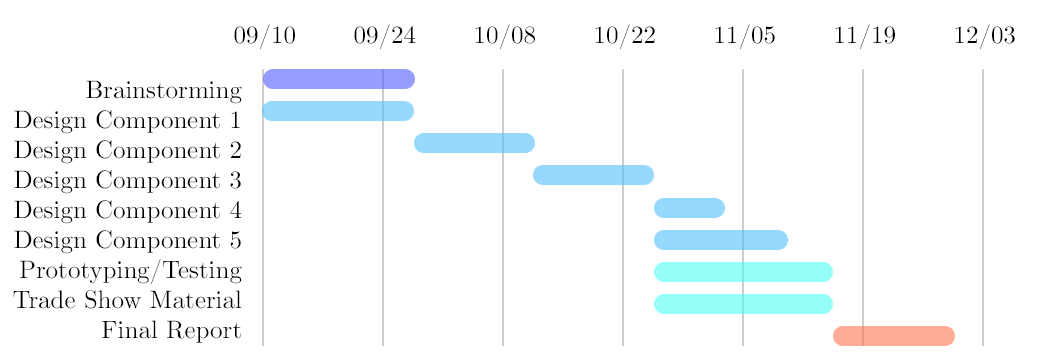
\includegraphics[width=0.75\textwidth]{motivation/gantt-psd-2.png}
    \caption{Gantt Chart for the VDBand Timeline 2018}
    \label{fig:gantt}
\end{figure}

\subsection{Methodology}
The approach used for this project is based on the parameters of pressure increase and inflammation to detect varicose veins. According to literature, the hydrostatic pressure has a difference of 90mmHg between two points in the same vein, while in the standing position \cite{press, press2}. It  also shows a temperature difference of 0.5\degree C \cite{Shaydakov}. These differences are the basis behind the detection system of the product. \\

In order to solve the aforementioned muscle issue in the calf, the team chose to use neuromuscular electrical stimulation (NMES). It is a widely used technique for any muscle application including pain management, decreasing atrophy, increasing range of motion, and improving muscle strength \cite{Doucet}. Hence, this is the treatment route that the project was based around. \\

The summary of this project is that once the detection system sees that varicose veins is present based on the differences mentioned above, the output would be the NMES on the calf until the symptoms are relieved to a comfortable level. 

\subsection{Socio-economic Impact}
Creating an instrument to aid patients with varicose veins would change lives in a significant way. Managing the discomfort of the disease is fairly difficult because there aren't many mitigating products to do so. Patients would often come home from work and elevate their legs, which prevented them from completing tasks which need to be done at home. This impacts not only the livelihood of a patient, but also the family dynamic in the household, as it puts added pressure on the patient as well as loved ones \cite{JCN}. For some patients, working was also difficult, as the leg had to be elevated, hindering their professional work \cite{JCN}.\\

Compression stockings were also an option, but were not preferred by patients, as they were considered "ugly and difficult to put on and wear" when they began wearing them. However, it did provide significant relief, so they got used to wearing them \cite{JCN}. Hence, creating a comfortable and easily accessible instrument would be a goal in this project. \\

Varicose veins also causes emotional and social pain, as many patients' decisions and priorities were altered due to the presence of their varicose veins. They had to make lifestyle changes due to pain or other effects from varicose veins, as well as a negative self-image due to the varicose veins \cite{JCN}. For example, patients may have to give up their leisurely activities that they used to participate in. When this involves activities with friends and loved ones, the decision to opt out of these activities can be difficult and they experience a sense of isolation \cite{JCN}. As mentioned before, varicose veins can also create low self-esteem, as patients are reluctant to show their legs in public due to the appearance of their legs. For some patients, the problem was more a psychological problem within themselves, as the feeling of being watched and judged was always in the back of their minds \cite{JCN}. This has a significant impact on mental health, which is a very important problem nowadays. Hence, a mitigation system for this may improve physical, social, and mental health.\\

In terms of economic impact, a study was done in the United Kingdom (UK) on the costs associated with varicose veins. All figures are in \pounds, which is the currency in the UK, at rates during the year of 2013. The costs associated with varicose veins can be seen in Table \ref{tab:Costs}. A specific cost according to Franz and Wann-Hanson is the cost of bigger shoes due to swelling feet, which can make it difficult during snow season, as it cause significant discomfort. This is a form of conservative care, which is why there are no treatment costs. The costs associated with conservative care throughout the year is associated to other therapeutic treatments which don't involve surgery \cite{UK}, which is why there are no costs for initial and recurring treatments, but there is one for total costs, in Table \ref{tab:Costs}.

\begin{table}[H]
    \centering
    \caption{Costs Associated with Treatment of Varicose Veins \cite{UK}}
    \vspace{3mm}
    \begin{tabular}{cccc}
    \hline
         Treatment & Initial Treatment (\pounds) & Recurring Treatment (\pounds) & Total Cost (\pounds)\\
         \hline
         Conservative Care & NONE & NONE & 1,102\\
         Surgery & 924 & 299 & 1,222\\
         Foam Sclerotherapy & 378 & 340 & 718 \\
         Endothermal & 639 & 230 & 869\\
    \hline
    \end{tabular}
        \label{tab:Costs}
\end{table}

\section{Literature Review}
For a disease with such a high prevalence in the United States alone, there is a surprisingly low amount of research associated with varicose veins. Nonetheless, a comprehensive literature review was performed to drive our team towards a new solution to a problem that affects over 50\% of people over the age of 50 \cite{Sell}.

\subsection{Treatment of Varicose Veins}
As previously mentioned in Section \ref{treatopt}, there are many treatment methods for varicose veins but the majority of them are invasive. Most patients today end up on the receiving end of a vein stripping or crossectomy procedure, which are considered the accepted standard procedure \cite{Willenburg}. However, Fischer et al. followed up on his patients 34 years after performing crossectomy and stripping of the great saphenous vein (GSV) and discovered clinical recurrence of varicose veins in more than half of those patients \cite{Willenburg}. These findings have driven the development of less invasive treatment modalities and surgery is being challenged in its role as a golden standard for treatment. \\

As a result, less invasive techniques using laser and radiofrequency were described in 2001 and 2000 respectively. In the first method, collagen shrinkage and fibrotic sealing of the vein lumen is induced by converting laser energy to heat. Important considerations such as the lengths of the waves, their delivery mode (continuous and pulsed), the radiation mode from the laser tip (radial and non-radial), and the material of the tip (bare fibre or gold tip) impact the destroying energy on both the treated vein and the surrounding tissue \cite{Willenburg}. Similarly, in endothermal radiofrequency ablation, heat is generated by radio waves, a type of electromagnetic radiation surrounding the active electrode. These electrodes had direct contact with the venous wall and emitted high radiofrequency energy. The produced electric current between these electrodes runs through the venous wall tissue generating heat \cite{Willenburg}. \\

Of these methods, compression therapy and the use of venoactice drugs are the only clinically viable non-invasive treatment methods that are currently used. Although there is no clear evidence that compression therapy slows down venous disease progression, it is seen to reduce venous hypertension, reflux, oedema, and improves the effectiveness of the calf muscle pump, there is even some evidence for the reduction of diurnal leg volume under compression therapy [Willenburg, Sell]. From a purely clinical perspective, varicose veins is exacerbated by an increase of trans-mural pressure on the vein walls so the goal of compression is that restore the trans-mural pressure to normal ranges by increasing the perivenous tissue pressure \cite{Rohan}.\\

In a study by Rohan et al. a patient-specific finite-element model of the human leg was developed to model the stress distribution in and around a vein wall in order to determine the biomechanical response of varicose veins to compression treatment. By inflating the sock and activating contact conditions between the skin and the compression sock, the initial stress on the vein wall was found through calculating the equilibrium position. As a result, it was found that the biomechanical response of veins are subject to three main factors: vein size, local radius of curvature, and the fat stiffness \cite{Rohan}. From these mechanical factors, one can appreciate the strong patient-specific response of the leg to external pressure and the potential effectiveness of this method of treatment. It was also found that the narrowing of the veins was less pronounced in the standing position which can be attributed to the fact that the applied external pressure has to work against the higher internal blood pressure \cite{Rohan}. 

\subsection{Detection of Varicose Veins}
There are several methods of detecting varicose veins that are currently being used clinically or being researched. Although clinical examination by a medical professional is generally the most widely accepted method, there is also thermography, fluoroscopy, and doppler ultrasound that may potentially be equally or more effective. Thermography uses an infrared camera to measure or detect the changes in heat patterns and blood flow in the body's tissues, fluoroscopy uses a continuous x-ray beam to study moving body structures, and Doppler ultrasound is an ultrasound technique that allows the doctor to see and evaluate blood flow through arteries and veins.

\begin{table}[H]
	\centering
	\caption{Detection rate of varicose veins for each method \cite{Gunn}}
	\vspace{3mm}
	\begin{tabular}{cccc}
	\hline
		Method & Veins Detected & Total Veins & Detection Rate \\
	\hline
        Clinical Examination & 73 & 135 & 54\% \\
        Thermography & 86 & 135 & 62\% \\
        Fluorography & 63 & 135 & 47\%\\
	\hline 
		\end{tabular}
		\label{table:detection}
\end{table}

\begin{table}[H]
	\centering
	\caption{False positive rate for each detection method \cite{Gunn}}
	\vspace{3mm}
	\begin{tabular}{cccc}
	\hline
		Method & False Positives & Total False Positives & False Positive Rate \\
	\hline
        Clinical Examination & 26 & 67 & 32\% \\
        Thermography & 26 & 67 & 32\% \\
        Fluorography & 30 & 67 & 36\%\\
	\hline 
		\end{tabular}
		\label{table:fpv}
\end{table}

From Table \ref{table:detection} it can be seen that the detection rate for thermography is greater, at 62\%, to that of a clinical examination performed by a doctor, which was 54\%, while fluoroscopy falls slightly behind both methods at 47\%. It can also be observed from Table \ref{table:fpv} that fluoroscopy has the highest false positive rate (36\%), whereas thermography and clinical assessment is tied at 32\%. As a result, thermography was our primary approach towards the detection of varicose veins.\\

Infrared thermography works on the principle that any matter with a temperature higher than absolute zero has thermal energy associated with it in the form of the kinetic energies of randomly moving atoms and molecules. These moving particles of a different charge generate electromagnetic fields resulting in the emission of photons, so an increase of temperature also increases the emission of infrared radiation from the surface of the body \cite{Shaydakov}.

\begin{figure}[H]
    \centering
    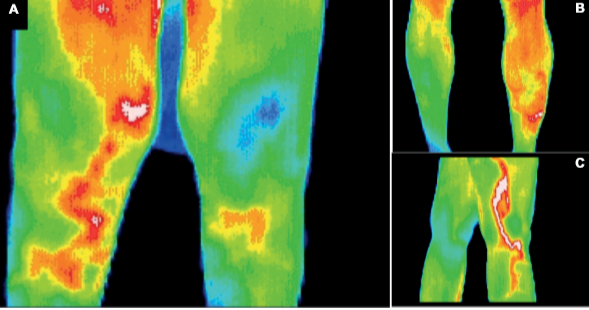
\includegraphics[width=0.7\textwidth]{litreview/thermograph.PNG}
    \caption{Thermogram of lower extremities displaying varicose veins \cite{Shaydakov}}
    \label{fig:vv_thermo}
\end{figure}

As seen in Figure \ref{fig:vv_thermo} panel A, the normal thermogram of the resting leg on the right appears as a relatively homogenous signal with a gradual decrease in infrared emission from the groin down to the foot. Generally, this signal does not exceed a temperature differential of more than 0.2\textdegree C to 0.3\textdegree C, so an increased local surface temperature of greater than 0.5\textdegree C, compared to the contralateral side, indicates a pathological process such as varicose veins \cite{Shaydakov}.\\

The increased temperature can be attributed to a mixture of inflammation and increased blood flow to the superficial veins that relieves venous obstruction. With a sensitivity and specificity of 80\% and 70\% respectively, there are several theoretical advantages to using thermography for the detection of varicose veins including low cost, speed of diagnostics (producing temperature readings in milliseconds), and high reproducibility, all while lacking the need for trained personnel \cite{Shaydakov, Usamentiaga}. 

\subsection{Neuromuscular Electrical Stimulation (NMES)}
Neuromuscular electrical stimulation (NMES) is a versatile tool that has many uses that range from strength training for athletes, rehabilitation for partially or completely immobilized patients, or even as a testing tool for neural or muscular function; but it is generally used to stimulate nerves and muscles to achieve a therapeutic response \cite{Herbert}. There are several electrical parameters that are particularly relevant to the use of NMES in the clinical setting and must be carefully considered, listed below, wherein some can be adjusted by the clinician to produce different treatment effects.

\begin{itemize}
    \item \textbf{Current} is produced by a flow of electrons that occurs when an electromotive force is applied to a closed circuit. Due to its nature, current is directional and can be described as either direct current, where it flows constantly in one direction, or alternating current, where it repeatedly changes direction. Most electrotherapy equipment, including NMES devices, outputs a biphasic current, which is essentially a direct current that has two phases (positive and negative) during each impulse, giving the effect of a net zero direct current. This protects the tissues from a build-up of electrochemicals, while allowing effective stimulation of the tissues \cite{Herbert}.
    \item \textbf{Resistance} is the slowing down of current due to material properties. Conductive materials that allow the current to move more freely are said to have a low resistance while materials that slow down the flow of current is said to have a high resistance. Resistance can cause a problem at the interface between the electrode and the skin as the skin has high resistance and is also well supplied with sensory nerve endings, making it difficult to input sufficient electrical energy into the tissues without the sensation becoming unbearable for the patient \cite{Herbert}. 
    \item \textbf{Ohm's Law} describes the relationship between the current, resistance, and voltage. This equation has a lot of clinical significance since skin resistance will change when the patient is moving, which means this will have a direct effect on the current or voltage.
    
    \begin{equation}
        V = I \cdot R
    \end{equation}
    
    If the voltage is fixed, any decrease in resistance in the circuit will produce an increase in the current to maintain the set voltage, this could result in a sudden peak of current that could be uncomfortable or even harmful to the patient’s tissues. Whereas a fixed current will produce a change to the voltage when there is any change to the resistance to keep the current at a constant level. Since the current level is responsible for the physiological effect of NMES, it is preferable to fix the current \cite{Herbert}. 
    \item \textbf{Intensity} refers to the amount of energy in the circuit, so in a clinical setting this is the amount or magnitude (amplitude) of energy being delivered to the patient's tissues. To be clinically effective the electrical stimulus used for NMES needs to be of sufficient intensity and of sufficient duration to depolarize the nerve membrane \cite{Doucet}. The intensity of stimulation varies for each individual, and is affected by oedema and moisture, so it is advised for patients to use a setting that is comfortable \cite{Ravikumar}.
    \item \textbf{Frequency} is the number of electrical impulses delivered in a given period of time and is measured in hertz (Hz) or cycles per second. For NMES, frequency is chosen to produce the desired effect within the tissues after an assessment of the patient. 1-10Hz is generally used for pain treatment, slow muscle fibres respond to 10-20Hz, and fast muscle fibres respond to stimulation frequencies of 30-60Hz \cite{Herbert}. Generally, a frequency range of 20-40Hz is used to achieve muscular contraction in a clinical setting.
    \item \textbf{Pulse Duration} refers to the length of time that each electrical pulse lasts for, usually measured in milliseconds (ms) or microseconds ($\mu$s), and \textbf{duty cycle} refers to the ratio between pulse delivery and rest. To prevent the muscle fibres becoming over-fatigued, the off time or rest phase will allow the motor units (consisting of a motor neuron and innervated muscle fibres) to repolarize and recover \cite{Herbert}.
\end{itemize}

With these considerations in mind, NMES has been shown in healthy individuals to increase venous blood flow parameters by artificially activating the calf-muscle pumps of the lower limb \cite{Ravikumar}. Additionally, with quotidian usage, muscle tone and strength can be improved within 12 weeks, which also improves blood flow in the lower extremities \cite{Son}. Therefore, the use of NMES for varicose veins can have both short-term and long-term benefits, especially when mixed with a more active lifestyle.\\

There are several studies that attest to the benefits of NMES. One such study by Son et al. stimulated the biceps two times per week for 12 weeks for 30 min at a time. The study measured isometric elbow flexion torque and biceps brachii muscle thickness both before and after training as evaluation metrics, and were measured at pre- and post-training. The study found that after the 12-week training period, the maximum isometric flexion torque increased by approximately 23\% compared to the initial performance \cite{Rohan}. Generally, there is a significant correlation (r=0.59; P$<$0.01) between muscle strength and muscle cross sectional area (CSA) in men, as seen in Figure \ref{fig:strvscsa} \cite{Maughan}. A similar relationship was also observed in women (r=0.59; P$<$0.01) \cite{Maughan}.

\begin{figure}[H]
    \centering
    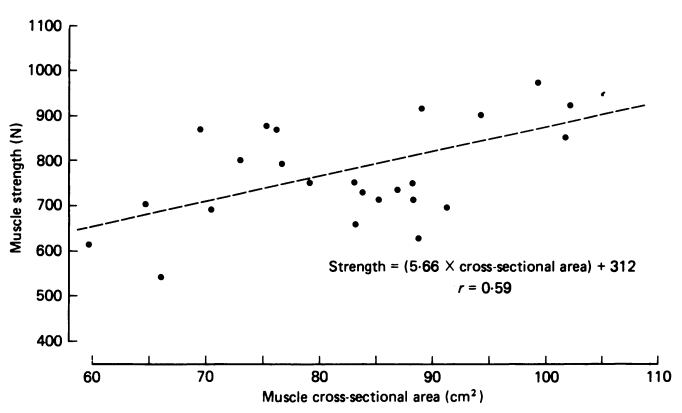
\includegraphics[width=0.6\textwidth]{litreview/csavsstr.png}
    \caption{Relationship between strength and CSA of the knee extensor muscles for males \cite{Maughan}}
    \label{fig:strvscsa}
\end{figure}

The study by Son et al. also found that muscle thickness at rest increased by approximately 8\% and 16\% at maximum voluntary contraction. This demonstrates the significant increase in muscle thickness on the trained vs. untrained side over the 12-week period (P$<$0.01), denoting the strength benefits of NMES \cite{Son}.\\

Although there are numerous benefits to the use of NMES, there are also a few limitations that may deter its use. Excessive neuromuscular fatigue is the more important limitation and has many causes but researchers are currently studying frequency, pulse width, modulation of pulses, amplitude, electrode placement, and the use of variable frequency pulse patterns to determine if fatigue can be reduced \cite{Doucet}. Another limitation is that muscle fibres are all simultaneously stimulated with NMES which is not the case during normal voluntary muscle contraction. As a result, the human motor system tries to offset fatigue by increasing the firing rate of active motor units and recruiting new motor units to replace others that have been derecruited, producing sudden, sometimes uncoordinated movement patterns \cite{Doucet}.\\

Even with these limitations, a clinical trial by Ravikumar et al. investigated the use of NMES in treating patients with venous disease. Measuring time-averaged peak velocity, peak venous velocity, and volume flow, a significant difference (P$<$0.0001) in the percentage change in vein flow parameters as well as limb volume increase between the NMES group and a sham group while using the device was found \cite{Ravikumar}.

\begin{figure}[H]
    \centering
    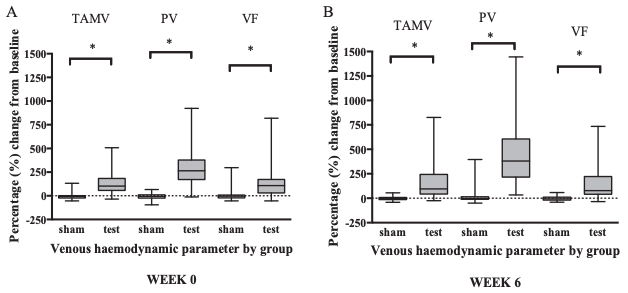
\includegraphics[width=0.7\textwidth]{litreview/wk0wk6.png}
    \caption{Percentage change in venous haemodynamics from baseline for groups at Week 0 and 6 \cite{Narayana}}
    \label{fig:strvscsa}
\end{figure}

\subsection{Compression Sleeve Design}
Compression therapy for patients with chronic conditions like varicose veins requires proper and adequate levels of compression in order to be effective while maintaining breathability and comfort at the same time. This has proven to be a challenges to health practitioners and compression sleeve manufacturers even to this date. As such there is a need for research in this field.\\

There are several modalities available for compression therapy such as bandage, stockings, and intermittent pneumatic compression (IPC) pumps. The bandage and stockings provide static compression and IPC devices provide dynamic compression. Although compression sleeves and stockings are considered the gold standard for compression therapy, there are noteworthy shortcomings that may lead to compromised treatment. As per the Centre Europeen de Normalisation (CEN) standard, there are several classes of compression being used as follows: light (Class-Ccl A: 10–14 mmHg), mild (Class-I: 15–21 mmHg), moderate (Class-II: 23–32 mmHg), strong (Class-III: 34–46 mmHg), and very strong (Class-IV: ≥49 mmHg) \cite{Narayana}.\\

Generally, compression sleeves are made of textile fibres including PET, Nylon, Cotton, Viscose, and Elastane, which all experience stress-relaxation over time in a stretched state, thus resulting in a drop of pressure \cite{Narayana}. Aside from this phenomenon, other material characteristics like elasticity, stiffness, and hysteresis can also affect how the sleeve behaves in both static and dynamic conditions over a prolonged period of time \cite{Narayana}. Therefore, it is very difficult to achieve target pressure with different leg attributes (shape and size), difference in materials (sleeve and leg), and time and temperature dependence \cite{Narayana}.\\

Although initially we had hoped to achieve dynamic pressure control to achieve a massage-like effect to improve blood flow, it became apparent that except for IPC, which can control pressure dynamically through pneumatics, there was no means for pressure control with a passive approach. To achieve the Goldilocks principle, there is currently research exploring the use of stress-memory polymeric filaments to achieve `smart stockings' that can dynamically control pressure without the noise, bulk, cost, and immobility of IPC units. Narayana et al. was able to achieve a massaging effect using memory filaments to store and retrieve stress in the presence of heat stimulus using a nylon single jersey plain knit structure with a stress-memory filament inlay as seen in Figure \ref{fig:stressmem}. This new technique was not incorporated into the design of the VDBand due to lack of testing and resources.

\begin{figure}[H]
    \centering
    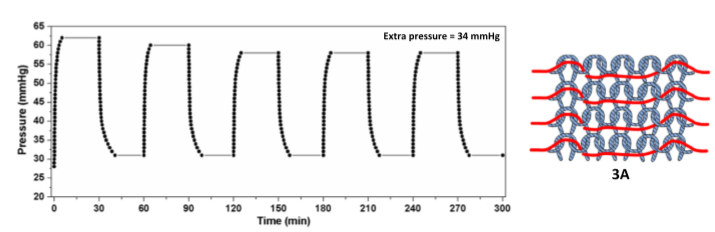
\includegraphics[width=0.75\textwidth]{litreview/stressmem2.PNG}
    \caption{Controlling massage effect via stocking structure and heat stimulus \cite{Narayana}}
    \label{fig:stressmem}
\end{figure}

\section{Business/Market Analysis}
\subsection{Current Market and Competitors}
There are many companies in the market that produce compression leg sleeves for different purposes and with different target markets. Leg compression sleeves can be made for athletes to aid in muscle recovery and provide extra calf support with manufacturers such as Zensah and shockdoctor \cite{Zensah}. However, there are compression sleeves that are geared towards helping reduce the symptoms of varicose veins with manufacturers such as OrthoSleeve. There are other methods of treatment to help treat varicose veins such as Sclerotherapy and Surgery, which are both invasive methods \cite{Mayo}. Currently in the market there are many products that claim to reduce the symptoms of varicose veins such as Antistax capsules which contain natural red vine leaf extract \cite{Antisatax}. Neuromuscular electrical stimulation compression sleeves were thoroughly researched in order to determine whether there were other products in the market similar to the VDBand. It was found that in the market there is an upper extremity biosleeve produced by the company AxioBionics, which contains electrical stimulation to aid muscle spasms, pain relief and muscle therapy in the arms and hands \cite{Axio}. A product idea currently in the market is a mobile therapeutic compression device that helps relieve pain in the lower back and calf muscles and improve circulation \cite{ACBJ}. These products are some of the main competitors. However, there is currently no product in the market geared towards reducing the symptoms of varicose veins in the lower extremities in the body that contains neuromuscular electrical stimulation. 

\subsection{Target Market}
The target market for the VDBand are adults, people that are overweight and pregnant women. In the Unites States, statistics show that one in four adults have varicose veins and that pregnant women and people that are overweight are more commonly affected by varicose veins since they have more pressure on their circulatory system \cite{MedNews}. Women are also four times more likely to have varicose veins than men and statistics show that one in two people over the age of 50 have varicose veins, which shows that older adults are more at risk \cite{Healthy}. Society has pressured everyone to look a certain way, and varicose veins is not only a medical concern but is a cosmetic issue for some. For those that are concerned about varicose veins being a cosmetic issue are also targeted since they will most likely want to reduce the visual appeal of the veins protruding. As for demographic factors, the United States is one of the largest markets since they have a large amount of people that are overweight. Since the VDBand is at an affordable price, economic factors don't play a large role. People that are less wealthy may find that the VDband is a little pricey, however those that are more wealthy will find it very affordable.   

\subsection{Cost Analysis}
\subsubsection{Manufacturing}
A comparison was performed to compare the costs of opening a manufacturing facility to produce the VDBand and the costs to get another company to manufacture the VDBand. If the company were to manufacture the VDBand, the start up costs and company costs for the very first month would be \$93,000. The breakdown of costs can be seen below in Table \ref{table:SCCC}.\\

The start-up and company costs for the first one-month time period include both fixed and variable costs. The lease, equipment and salary expenses are fixed costs and the electricity, hydro, renovation, legal and contingency are variable costs since the costs depend on a variety of factors. 

\begin{table}[H]
	\centering
	\caption{Start Up Costs and Company Costs for the First Month}
	\vspace{3mm}
	\begin{tabular}{cc}
	\hline
		Start Up Costs and Company Costs & Cost(\$) \\
	\hline
		Lease & \$1,000 \\
	    Electricity  & \$1,200 \\
		Hydro & \$1,100\\
		Equipment & \$30,000 \\
		Renovation & \$10,000\\
		Legal & \$15,000 \\
		Salary Expense & \$30,000 \\
		Contingency & \$5,000 \\
		\hline
	    Total Cost & \$93,300 \\
	 \hline 
		\end{tabular}
		\label{table:SCCC}
\end{table}

The company costs for a one-month period starting at the second month have all the same costs as the first month except the equipment, renovation and legal costs. These costs have already been paid for and don’t need to be re-paid each month. In the future, the company costs per month can change for a variety of reasons, such as an increase in salary of a manager. This would increase the overall monthly costs. Since the company is planning to expand, there will be an increase in workers in the future which will increase salaries expensive and efficiency. Every month after the first month would accumulate a cost of \$37,400, which can be seen below in Table \ref{table:CCPM}. This means that the total start-up costs would be \$54,500.

\begin{table}[H]
	\centering
	\caption{Company Costs for a One-Month Period}
	\vspace{3mm}
	\begin{tabular}{cc}
	\hline
		Company Costs & Cost(\$) \\
	\hline
		Lease & \$1,000 \\
	    Electricity  & \$1,200 \\
		Hydro & \$1,100\\
		Equipment & \$30,000 \\
		Salary Expense & \$30,000 \\
		Contingency & \$5,000 \\
	\hline
	    Total Cost & \$37,400 \\
	 \hline 
	\end{tabular}
	\label{table:CCPM}
\end{table}

If the company were to get another company to manufacture the product, it would cost \$59,500 each month. This is an extra \$22,100 each month, which in turn would add up to a lot of money. The other company would have to also purchase all the components, packaging and would charge for labour and production costs. The breakdown of these costs is shown in Table \ref{table:OCC}.

\begin{table}[H]
	\centering
	\caption{Cost of Another Company Manufacturing the VDBand Over a One-Month Time Period}
	\vspace{3mm}
	\begin{tabular}{cc}
	\hline
		Costs & Cost(\$) \\
	\hline
		Components & \$18,000 \\
	    Labour & \$40,000 \\
		Packaging Costs & \$500\\
		Production Costs & \$1,000 \\
	\hline
	    Total Cost & \$59,500 \\
	 \hline 
	\end{tabular}
	\label{table:OCC}
\end{table}

Starting up the company takes time, effort and money, A cost analysis was performed and it was evident that it would be more cost efficient for the company to open up a manufacturing facility to mass produce the product instead of providing it to another company. For the first month, the start up and company costs would be more expensive than having another company manufacture the product, however in the long run it would be cheaper. The costs significantly increase over time and would not be beneficial for the company. The company begins with a negative profit, but drastically increases over the years. Figure \ref{fig:CPAG}. shows the profit of the company producing the product, cost for the company to produce the product and the costs associated with another company manufacturing the product.

\begin{figure}[H]
    \centering
    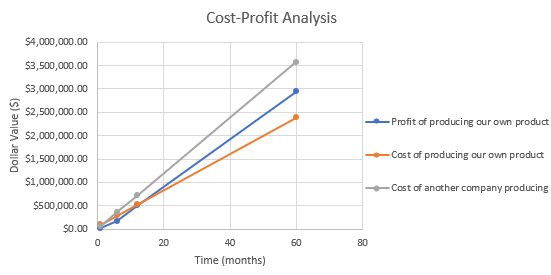
\includegraphics[width=1.0\linewidth]{marketing/CPG.PNG}
    \caption{Cost Profit Analysis.}
    \label{fig:CPAG}
\end{figure}
\vspace{0.5mm}

\subsubsection{Distribution}
The VDBand will be fully assembled and distributed in Canada with the components being outsourced from other companies. It will be cheaper for the company to outsource its components, than manufacturing every single component separately for the VDBand. This allows the mass production to be efficient and effective. The components will be purchases in bulk in order to lower costs, improve efficiency and increase profit margins. Manufacturing this product will be substantially more expensive than manufacturing in another country such as China, but to assure a high quality product, the company has chose to manufacture the product in Canada. The manufacturing facility will be located in Oakville, Ontario and will be used for assembly and distribution. The VDBand will begin distributing across North America for the first year and after a year distribute to other countries around the world. The company will start off small with a few people in upper management, engineers and marketing specialists. The company will continue to expand over the years and continue to improve its products. 


\subsubsection{Bill of Materials}
The VDBand contains minimal parts, is very small, compact and flexible. The total cost of one unit without considering manufacturing costs is \$57.86. Regular compression sleeves are usually around \$20 and contain no neuromuscular electrical stimulation. For another \$40, the VDBand provides both compression and neuromuscular electrical stimulation to aid in reducing varicose symptoms. The bill of materials displays all the parts of the sleeve and the cost of each part, and can be seen below in Table \ref{table:BOM}.

\begin{table}[H]
	\centering
	\caption{Bill of Materials}
	\vspace{3mm}
	\begin{tabular}{cccc}
	\hline
		Part Name & Number of Parts used & Cost per Part (\$) & Total Cost (\$) \\
	\hline
		Compression Sleeve & 1 & 10.00 & 10.00 \\
		Roll of Velcro  & 1 & 8.40 & 8.40 \\
		Force Sensitive Resistor (FSR 406) & 2 & 12.40 & 24.80 \\
		Thermistor (SEN00250) & 2 & 0.75 & 1.50 \\
		Electrical Muscle Stimulator Pads & 2 & 0.87 & 1.74\\
		10k\ohm Resistor & 2 & 0.30 & 0.60 \\
		5.6k\ohm Resistor & 3 & 0.30 & 0.90 \\
		Power MOSFET (IRFZ44N) & 4 & 1.67 & 6.68 \\
		9V Power Source & 1 & 1.89 & 1.89 \\
		Wires (1m) & 1 & 0.75 & 0.75 \\
	\hline
	    Total Cost &  & 37.63  & \textbf{57.86}\\
	 \hline 
		
	\end{tabular}
	\label{table:BOM}
\end{table}

\subsubsection{Material Cost Breakdown}

As mentioned previously, the components will be outsourced from other companies and ordered in bulk to reduce costs. Over time, the total material cost per product decreases since production costs decrease. As time increases, the cost of individual parts remain the same however the production costs decrease as more units are made. Table \ref{table:MCB} shows the material cost breakdown including packaging costs and productions costs over a five year period. 

\begin{table}[H]
	\centering
	\caption{Material Cost Breakdown over a 5 Year Period}
	\vspace{3mm}
	\begin{tabular}{ccccc}
	\hline
		Part Name & $1^{st}$ Month (\$) & 6 Months (\$) & $1^{st}$ Year (\$) & 5 Years (\$) \\
	\hline
		Compression Sleeve & 10.00 & 10.00 & 10.00 & 10.00 \\
		Roll of Velcro  & 8.40 & 8.40 & 8.40 & 8.40 \\
		Force Sensitive Resistor (FSR 406) & 24.80 & 24.80 & 24.80 & 24.80 \\
		Thermistor (SEN00250) & 1.50 & 1.50 & 1.50 & 1.50 \\
		Electrical Muscle Stimulator Pads & 1.74 & 1.74 & 1.74 & 1.74\\
		10k\ohm Resistor & 0.60 & 0.60 & 0.60 & 0.60\\
		5.6k\ohm Resistor & 0.90 & 0.90 & 0.90 & 0.90\\
		Power MOSFET (IRFZ44N) & 6.68 & 6.68 & 6.68 & 6.68\\
		9V Power Source & 1.89 & 1.89 & 1.89 & 1.89\\
		Wires & 0.75 & 0.75 & 0.75 & 0.75\\
		Packaging & 0.75 & 0.75 & 0.75 & 0.75 \\
		Production Costs & 4.00 & 3.50 & 3.00 & 1.50 \\
	\hline
	    Total Cost & 62.61  & 62.11  & 61.61 & \textbf{60.11}\\
	 \hline 
		
	\end{tabular}
	\label{table:MCB}
\end{table}

\subsubsection{Cost-Profit Analysis}
As mentioned previously, the cost of producing each unit is \$57.86, however the VDBand will sell at a retail price of \$175.00. This is a profit margin of about 300 percent, which allows for a reasonable profit per unit. Depending on the number of units sold, net income will vary and over time more units will be sold. The cost-profit analysis over a 5 year period can be seen below in Table \ref{table:CPA}.

\begin{table}[H]
	\centering
	\caption{Cost-Profit Analysis over a 5 Year Period}
	\vspace{3mm}
	\begin{tabular}{ccccc}
	\hline
		 {\hspace{1em}} & $1^{st}$ Month & 6 Months & $1^{st}$ Year & 5 Years \\
	\hline
		Manufacturing Cost & \$62.61 & \$62.11 & \$61.61 & \$60.11 \\
		Retail Price  & \$175.00 & \$175.00 & \$175.00 & \$175.00\\
	    Units Sold  & 200 & 1500 & 4400 & 25600 \\
		Cost of Goods Sold & \$12,522.00 & \$93,165.00 & \$271,084.00 & \$1,538,816.00 \\
		Net Income & \$35,000.00 & \$262,500.00 & \$770,000.00 & \$4,480,000.00\\
	
	\hline
	    	Profit & \$22,478.00 & \$169,335.00 & \$498,916.00 & \$2,941,184.00\\
	 \hline 
		
	\end{tabular}
	\label{table:CPA}
\end{table}

Over the years, profit will drastically increase since the manufacturing costs are decreasing and more units are being sold. This drastic increase is very apparent as seen above in Figure \ref{fig:CPAG}. The production costs will also decrease as cost for equipment and manufacturing will be paid off.

\subsection{SWOT Analysis}
One of the strengths of the VDband includes being different from other compression sleeves in the market, since it includes neuromuscular electrical stimulation, which allows it to be more marketable. One weakness would be that for those that are not as wealthy, \$175.00 would be fairly expensive, however it is a good investment for those with varicose veins. The VDBand provides a lot of different opportunities both for the company and for buyers. The company has the opportunity to sell to various countries and help those with varicose veins all around the world. The VDBand provides a great opportunity to many different people such as people that are overweight, and women that are pregnant that suffer from varicose veins. A threat that could occur is if a product is not manufactured properly and is faulty, it could potentially harm the person using the product since it has a lot of circuitry inside the sleeve. However, this is why the company will have a quality assurance department to ensure product safety and ensure the product is of high quality. 

\subsection{Marketing Strategy}
It is believed that one of the best ways to communicate with adults is through television. Even though web applications such as Netflix have become extremely popular, television is still largely watched with Americans watching more than 7 hours and 50 minutes per household per day \cite{ATL}. According to Statista, in Canada, adults spend about 24 minutes with print media, about 94 minutes listening to the radio and 202 minutes watching television \cite{Stats}. Older adults spend even more time watching television since they are usually retired and have more free time \cite{Stats}. This is beneficial for the company since the VDBand is geared towards older adults since they are more prone to getting varicose veins. \\

Commercials on television for the VDBand will reach out to adults all around the world on different channels and commercials will also play on a variety of radio stations. The commercial will run on television on weekdays from five to eight pm which is usually when adults get home from work and watch the news or television shows and on weekends from nine to twelve pm when adults usually wake up. The commercial will air on the radio on weekdays from six to nine am since that is when adults are driving to work and listen to the radio and on weekends from twelve to three pm when adults run errands. The commercial will be about 30 seconds long and consist of a demonstration of the VDBand and the benefits that are associated with the product will be described. The commercial will begin airing on radio stations and when enough profit is made, it will be aired on local television and then national television. A commercial on local television of about 30 seconds can cost two hundred dollars to \$1500 every time the commercial is aired and on national television it can cost around \$123,000 \cite{FSB}. These expenditures will be taken into account in the future when advertising expenses are determined. \\

The VDBand will also be displayed in printed media such as posters in malls, hospitals, doctors offices, community centres and in magazines such as the People and Entertainment Weekly. People tend to enjoy keeping tabs on their favorite celebrities and buy magazines to read about these celebrities, The top two celebrity magazines happen to be People and Entertainment Weekly \cite{AYCR}. Since the VDBand is a medical device, it will be advertised to doctors and hospitals and advertised to their patients, since this is a large target market. The VDBand will also be on internet ads and on social media platforms such as Facebook, Snapchat and Instagram. Adults tend to do a lot of webs surfing and more adults are using social media these days, so this would be a good way to reach out to the target market. For the future, the marketing department will come up with additional and better ideas for marketing the product.

\subsection{Advertisement}
Advertising plays a large role in the success in a company. The goal is to advertise the VDBand over a variety of platforms in order to hit a large portion of the market. As mentioned previously, posters will be displayed in hospitals and doctor’s offices, along with brochures that people can take home. This allows people to get a better understanding of the product and whether it is suited for their needs. Our informational brochure is available to the public and seen below in Figure \ref{fig:brochure}.\\

On the future brochures, the website for the company will be there for the public to find out more about the company and its beneficial products. For the future, the marketing department will come up with additional and better ideas for marketing the product. 

\begin{figure}[H]
    \centering
    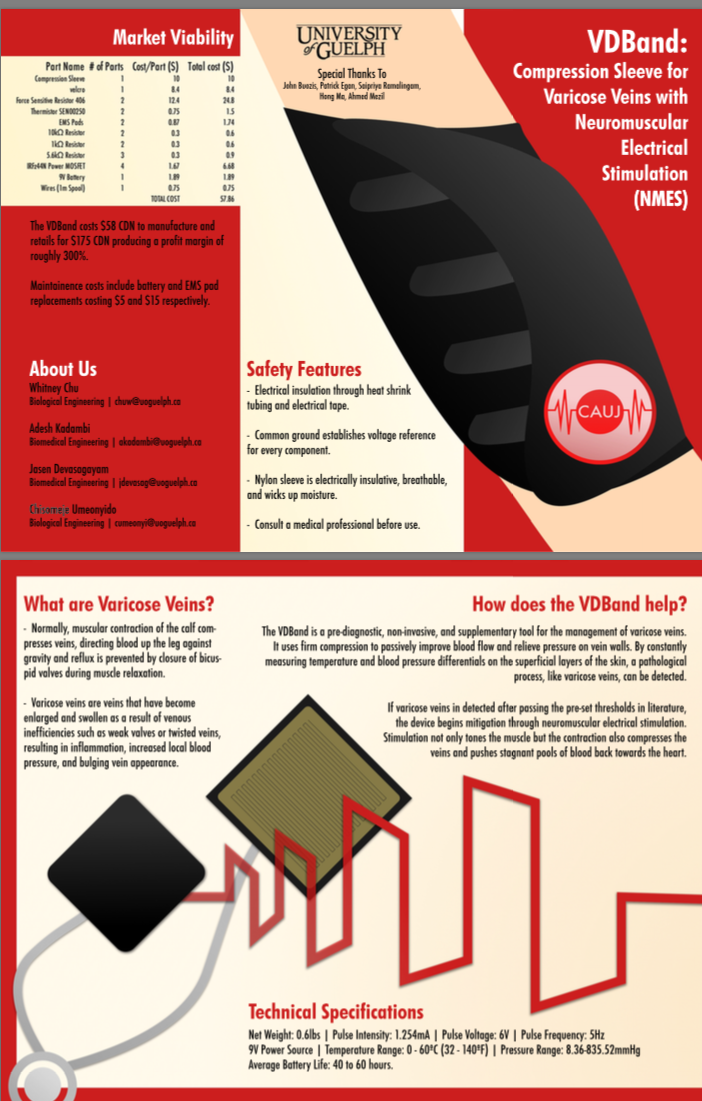
\includegraphics[width=0.8\textwidth]{marketing/brochure.png}
    \caption{Sample Brochure for the VDBand}
    \label{fig:brochure}
\end{figure}

\subsection{Product Life Cycle}
The product life cycle begins with all the raw materials outsource from other companies. Then product gets manufactured and assembled and then packaged. The products are put into storage until they are distributed. Once they are distributed, they are used by the public. When the components are worn out or broken, they can be sent back to the manufacturer to replace the parts required at a price. The issue of the product can be brought to the attention of the company and a price estimate will be given to decide if its better to replace the parts or for the buyer to buy a whole new product This begins the cycle again starting at manufacturing and assembly. If the product can no longer be fixed or have its parts replaced, the product hits its end of life. The end of life contains two parts: dispose of some raw materials and recycle some materials. Some components of the VDBand may be recycled and reused and other components need to be placed in the garbage. The full product life cycle of the VDBand can be seen below in Figure \ref{fig:PLC}. The VDBand has a decently long life-cycle, as long as the product is well kept, used properly and can be repaired if damaged.

\begin{figure}[H]
    \centering
    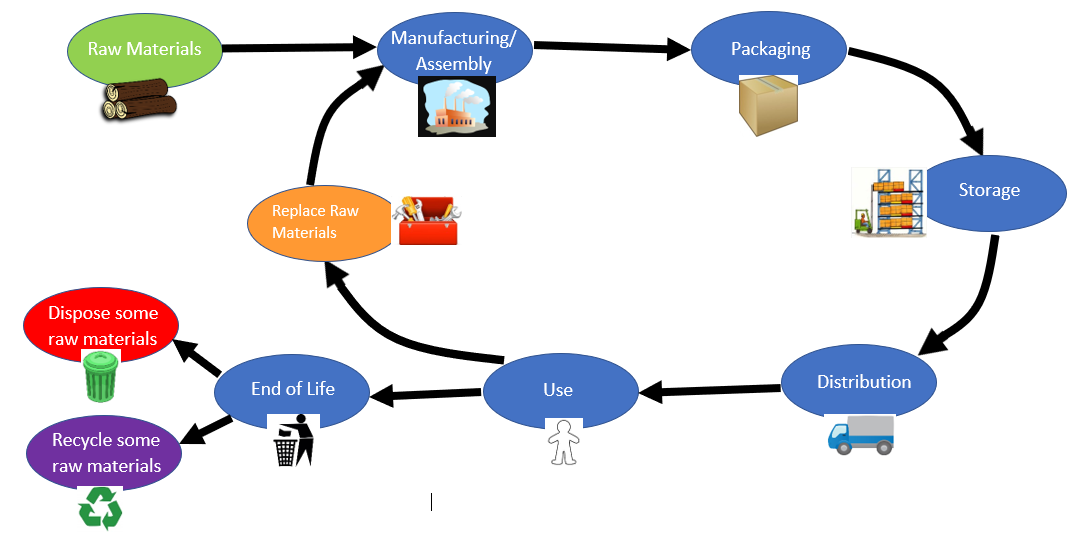
\includegraphics[width=1.05\linewidth]{marketing/PLC.PNG}
    \caption{Product Life Cycle}
    \label{fig:PLC}
\end{figure}

\subsection{Business Model Canvas}
A Business Model Canvas shows all the finance, value and goals of a company. The Business Model for CAUJ is shown below in Figure \ref{fig:BCM}. CAUJ includes key partners, key resources, key activities, customer segments, customer relationships, value propositions, channels, cost structure and revenue streams in the Business Canvas Model.

\begin{figure}[H]
    \centering
    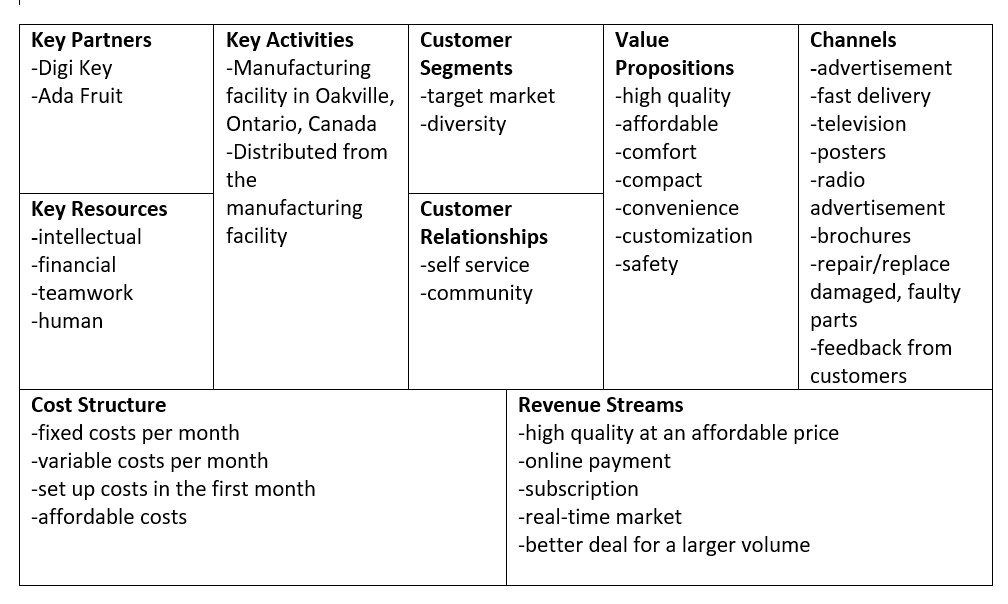
\includegraphics[width=0.8\linewidth]{marketing/BCM.PNG}
    \caption{Business Canvas Model}
    \label{fig:BCM}
\end{figure}

\section{Product Design}

%   Product advantages, Components and design, Design challenges, Design elements, Appearance and theme, Instructions, Testing prototype, Future design

\subsection{Design Elements}
Compression sleeves have saturated the market as support for varicose veins. In order to make an impact in the same market, there were many design elements and considerations that needed to be fulfilled. The primary aesthetic design considerations for the VDBand included providing adequate compression comparable to other commercial compression sleeves, ensuring sleeve breathability to prevent excessive sweating or buildup of heat, and ensuring a lightweight design to provide comfort and everyday usability. In order to satisfy these sleeve criteria, the best choice of material seemed to be nylon sleeves, as it is expandable, breathable, and commonly used to wick up sweat.\\

In addition to the aesthetic elements, there were many functional design elements that had to be considered to ensure product success. First, it had to have the ability to quantify surface temperature differential between afflicted area and healthy reference point. Since just one metric is unable to accurately detect varicose veins without a high false positive rate, our device needed to quantify blood pressure differential between afflicted area and healthy reference point as well.
Secondly, the device needed to be able to output an electrical pulse when the presence of varicose veins was detected. The waveform had to be a an amplitude and frequency that resulted in the contraction of the muscles, which would consequentially relieve the afflicted area of the accumulated blood. \\

The components of the electric circuit in the device are discrete components which are based on through hole technology. They are able to be mounted on a printed circuit board containing vias or a prototype perfboard. The circuit featured two thermistors, two force sensitive resistors, two 1 k\ohm resistors, five 1 k\ohm resistors, four N-channel power MOSFETS, and two EMS electrodes. The circuit was divided into three separate subsections: the input circuit which consisted of the sensors that were used, the microcontroller which was an AdaFruit Flora \textsuperscript{(TM)}, and the output circuit which consisted of an H-bridge that was able move the voltage across the electrodes between positive to negative values. Ther original circuit and final circuit can be referenced in Appendix A1 and Appendix A2. \\

The input circuit consisted of the sensor that would be used in the product. Each sensor was arranged in a voltage divider with a resistor for the voltage at their intersecting node to be read. The resistance of the sensors were able to vary with temperature and pressure which would result in a change in voltage at a node if they were placed in a voltage divider network. The change in resistance of both sensors is inversely proportional to the change in either the temperature or the pressure. The thermistor being used is referred to as a Negative Temperature Coefficient (NTC) thermistor, whose resistance decreases as the temperature it is subjected to increases and vice versa. The input-output conversion can be seen in Appendix A3. A logarithmic curve can be plotted showing the resistance of thermistor as a function of the temeperature, and this can be seen in \ref{fig:Therm}. An operating range of 0-60\degree C was chosen for the purpose of this project. The equation derived from \ref{fig:Therm} is used to convert the resistance of the thermistor into a temperature value, and that equation is 
\begin{equation}
T = \frac{log(R)-4.4646}{-0.01861}
\end{equation}
where $T$ = Temperature (\degree C) and $R$ = Resistance (\ohm).\\

A force sensitive resistor has a similar relation between its pressure it is subjected to and its resistance. Two thermistors and two force sensitive resistors were used to calculate a difference in temperature and blood pressure between two regions of the sleeve. One thermistor and one force sensitive resistor was placed at a point on the sleeve that would make contact with a non-afflicted region of the body, while the other two was positioned at a region that would make contact with the afflicted area.\\

\begin{figure}[!ht]
    \centering
    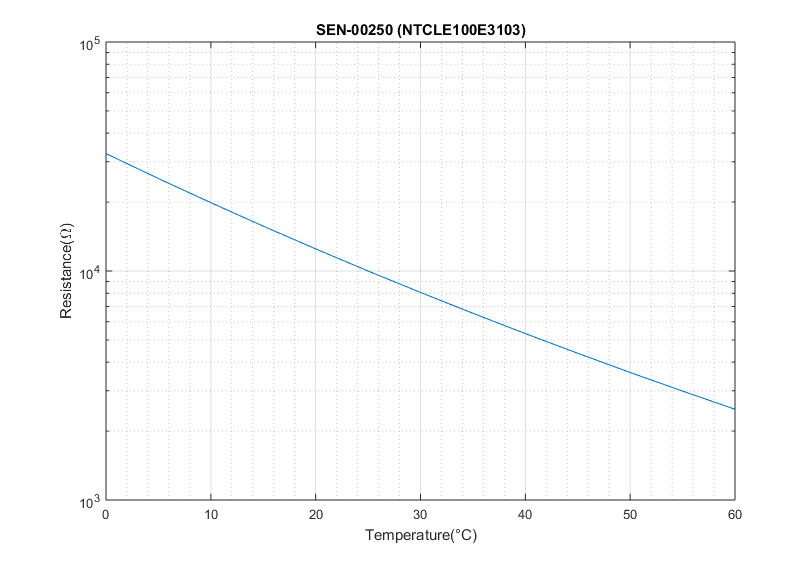
\includegraphics[width = 1.0\linewidth]{SEN00250.png}
    \caption{Logarathmic Curve for Thermistor (SEN00250)}
    \label{fig:Therm}
\end{figure}

The temperature and pressure difference of the afflicted and non-afflicted areas would be taken to determine whether varicose veins have occurred in the user. instead of measuring the elevated blood pressure and temperature directly in the afflicted area, the difference in these two parameters between a healthy and non-afflicted region was chosen to be evaluated. A single thermistor and force sensitive resistor will have an offset value because they will also be evaluating the temperature and pressure of the external environment, rather than only the skin of the user. There will also be noise inherent in the sensors. The difference in the parameters mitigates the offset value and the noise present in the sensors. The analog values will then be read by the Adafruit flora which has the same architecture as the Arduino Lilypad.\\

The Adafruit Flora features several digital and analog input and output pins, serial communication, I\superscript(2)C communication, Serial Peripheral Interfacing (SPI), and an output source that can deliver 3.3 V and 150 mA \cite{Ada}. The operating voltage of the controller is between 3.3 to 16 V, with reverse polarity protection. The Flora uses the ATmega 32u4 microcontroller developed by AVR, which operates at 8 MHz \cite{Ada}. The micro controller was chosen due to its small size and its flexibility. It is specifically used to design wearable technology. The Flora would receive information from the sensors in the form of analog signals, then once the requirements for varicose veins have been satisfied, the output circuit will activate, which will aid in the recovery process. The prototype of the sleeve contains the sensors, Flora, neuromuscular electrical stimulation pads and the arduino code. The protoype of the sleeve can be seen below in Figure \ref{fig:PTS}. 

\begin{figure}[H]
    \centering
    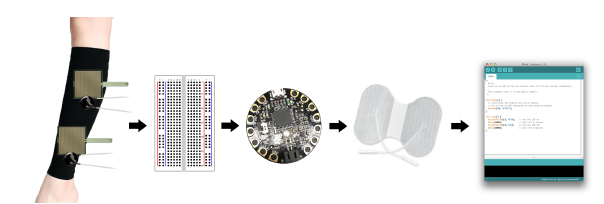
\includegraphics[width=0.7\linewidth]{design/PTS.PNG}
    \caption{Prototype Schematic}
    \label{fig:PTS}
\end{figure}
\vspace{0.5}

The output circuit consists of 4 transistors arranged as an H-Bridge, and two electrodes. The electrodes are attached to the output terminals of the H-Bridge, which allows for the current to reverse in direction when specific inputs are activated. The H-Bridge circuit is used to control the direction a motor shaft revolves by reversing the polarity of the voltage applied . The electrodes operate on the same principle, in that the voltage applied across them needs to be continually reversed to generate a square wave signal. When the pads are applied across the skin, the circuit will be closed which will allow for the muscles to contract. 

\subsection{Power Consumption of Circuit}
The input circuit's sensor is where most of the power consumption occurs. The circuit is supplied by a 9V battery, where 6V goes to the input circuit, as that is what is required to power the Flora. The remaining 3V supplies the NMES pads to produce the electrical muscle stimulation. The power consumption for all the components is shown below in \ref{table:power}.

\begin{table}[!ht]
    \caption{Power Consumption of Circuit Components}
	\vspace{3mm}
	\centering
	\begin{tabular}{cccc}
	\hline
		 Component & Supply Voltage (V) & Supply Current (mA) & Power Consumption (mW)\\
	\hline
		Adafruit Flora & 5.5 & 20 & 110\\
		Force Sensor &  5 &  5 &  25\\
        Thermistor &5   & 5 &  25\\
	\hline
	\end{tabular}
	\label{table:power}
	\end{table}

\subsection {Alternative Designs for Output Circuit}
The realization of the output circuit was a difficult obstacle for the group to overcome. The square wave was needed to cause a muscle contraction in the patient. Initially, a virtual ground was to be employed through the following circuit as seen in Figure 12. The circuit shifts the reference point at which the voltage readings are taken. In is able to make a 9 V power source to have an output voltage of +4.5V and -4.5V depending on where the input is read from. The square wave would have been able to be generated by switching which nodes the output voltage was read from, however this circuit is unreliable due to the drift that it inherent in the components. The voltage would start to vary over time at the  nodes due to the load that will be connected at the output. \\

\begin{figure}[H]
    \centering
    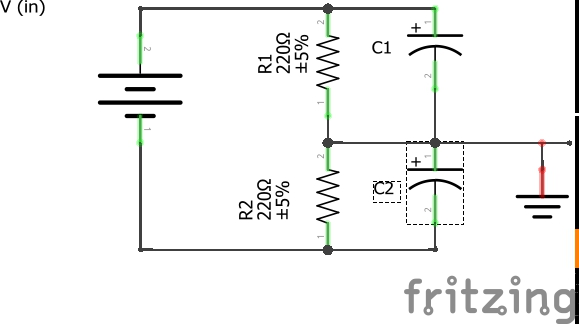
\includegraphics[width=0.55\linewidth]{Circuits/Circuit1.jpg}
    \caption{Initial Virtual Ground Circuit}
    \label{fig:PLC}
\end{figure}
\vspace{0.5}

The team also wanted to use a circuit featuring a transformer to generate the square wave, however the transformer can only operate on AC voltages. The initial input would a DC voltage from our microcontroller. The transformer would also aid unnecessary weight to the product which could have resulted in some discomfort for the consumer. \\

An amplifier circuit was considered by the team to increase the voltage level given as an input by the Flora, The flora is able to output a pulse width modulation signal that would function as a square wave. The signal would have been amplified by an Op-Amp arranged in a negative feedback configuration with a pre-calculated gain as seen in Figure 13. The team did not use this design for the square wave because  Op-Amp can only amplify something up to a certain negative and positive value. The Op amp would have its negative lead connected to ground since there was not a readily available negative voltage supply. The design for a negative voltage supply would have required further research and time.  \\

\begin{figure}[H]
    \centering
    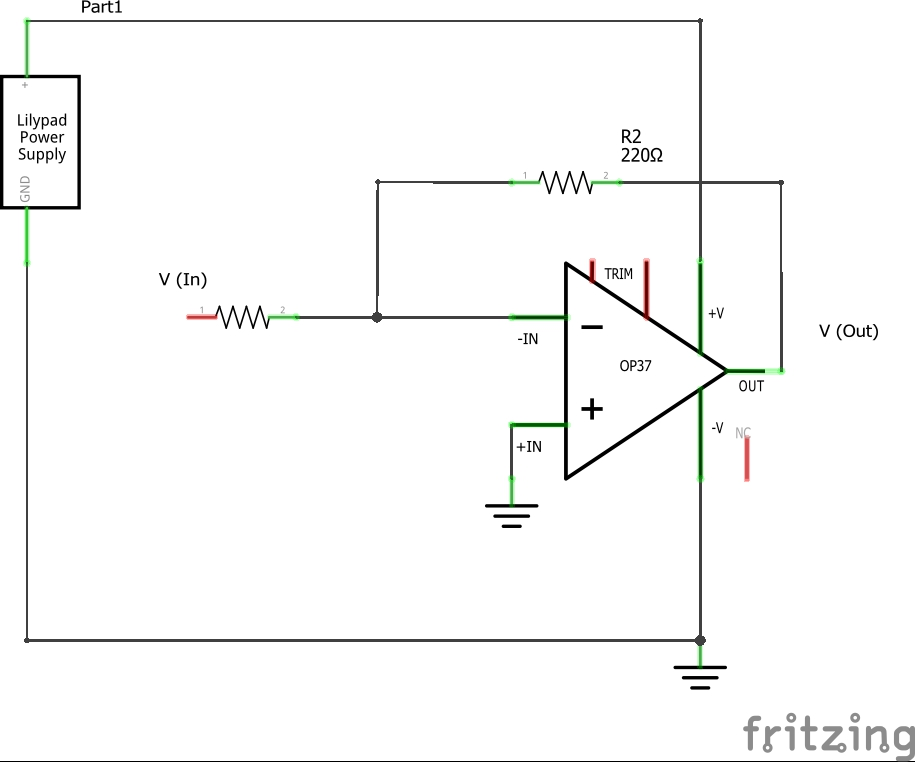
\includegraphics[width=0.55\linewidth]{Circuits/Circuit2.jpg}
    \caption{Amplifier Circuit}
    \label{fig:PLC}
\end{figure}
\vspace{0.5}

\subsection{Final Design}
The final design that was chosen by the group was the H-Bridge which consisted of four transistors as seen in Figure \ref{fig:PLC}. 

\begin{figure}[H]
    \centering
    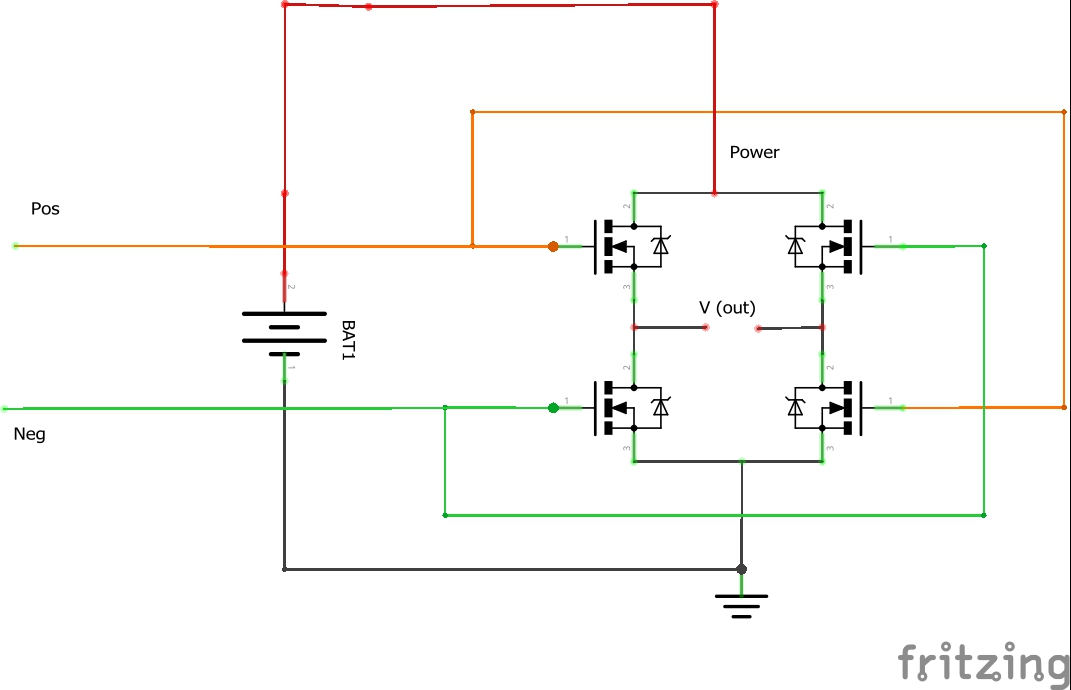
\includegraphics[width=0.55\linewidth]{Circuits/H-Bridge_schem.jpg}
    \caption{H-Bridge Circuit}
    \label{fig:PLC}
\end{figure}
\vspace{0.5}\\

They were all chosen to be N-Channel MOSFETS because of their high switching times, and the fact that they were only voltage controlled rather than current and voltage controlled like Bipolar Junction Transistors (BJT) \cite{All}. This provides the advantage of faster switching times, and also there is inherently less noise present in the system than there would be if BJTs were used. When the electrodes are connected to the output terminals of the H-Bridge, and placed on the skin of the consumer, the circuit will be closed. When the input labeled positive has a HIGH logic value applied to it, the transistors in the upper left and lower right sections turn on and create a positive voltage across the output terminals. If a HIGH logic level is applied to the input labeled neg, then the upper right and lower left transistors turn on and created a negative voltage. As the inputs are turned on and off at a specific frequency, a square wave is developed. Please refer to Appendix A3, section Output.ino to view how the square wave was generated. The compression sleeve itself is black and made of a nylon material. All the electrical components are sewn into the sleeve to prevent interaction with skin. Only the force sensitive resistors, thermistors and neuromuscular electrical stimulation pads make direct contact with the skin. The VDBand has velcro on it, making it adjustable to different calf sizes and the product itself is stretchy, comfortable and compact. The final product can be seen below in Figure \ref{fig:VDB} and the components used can be referenced in Appendix A5.\\

\begin{figure}[H]
    \centering
    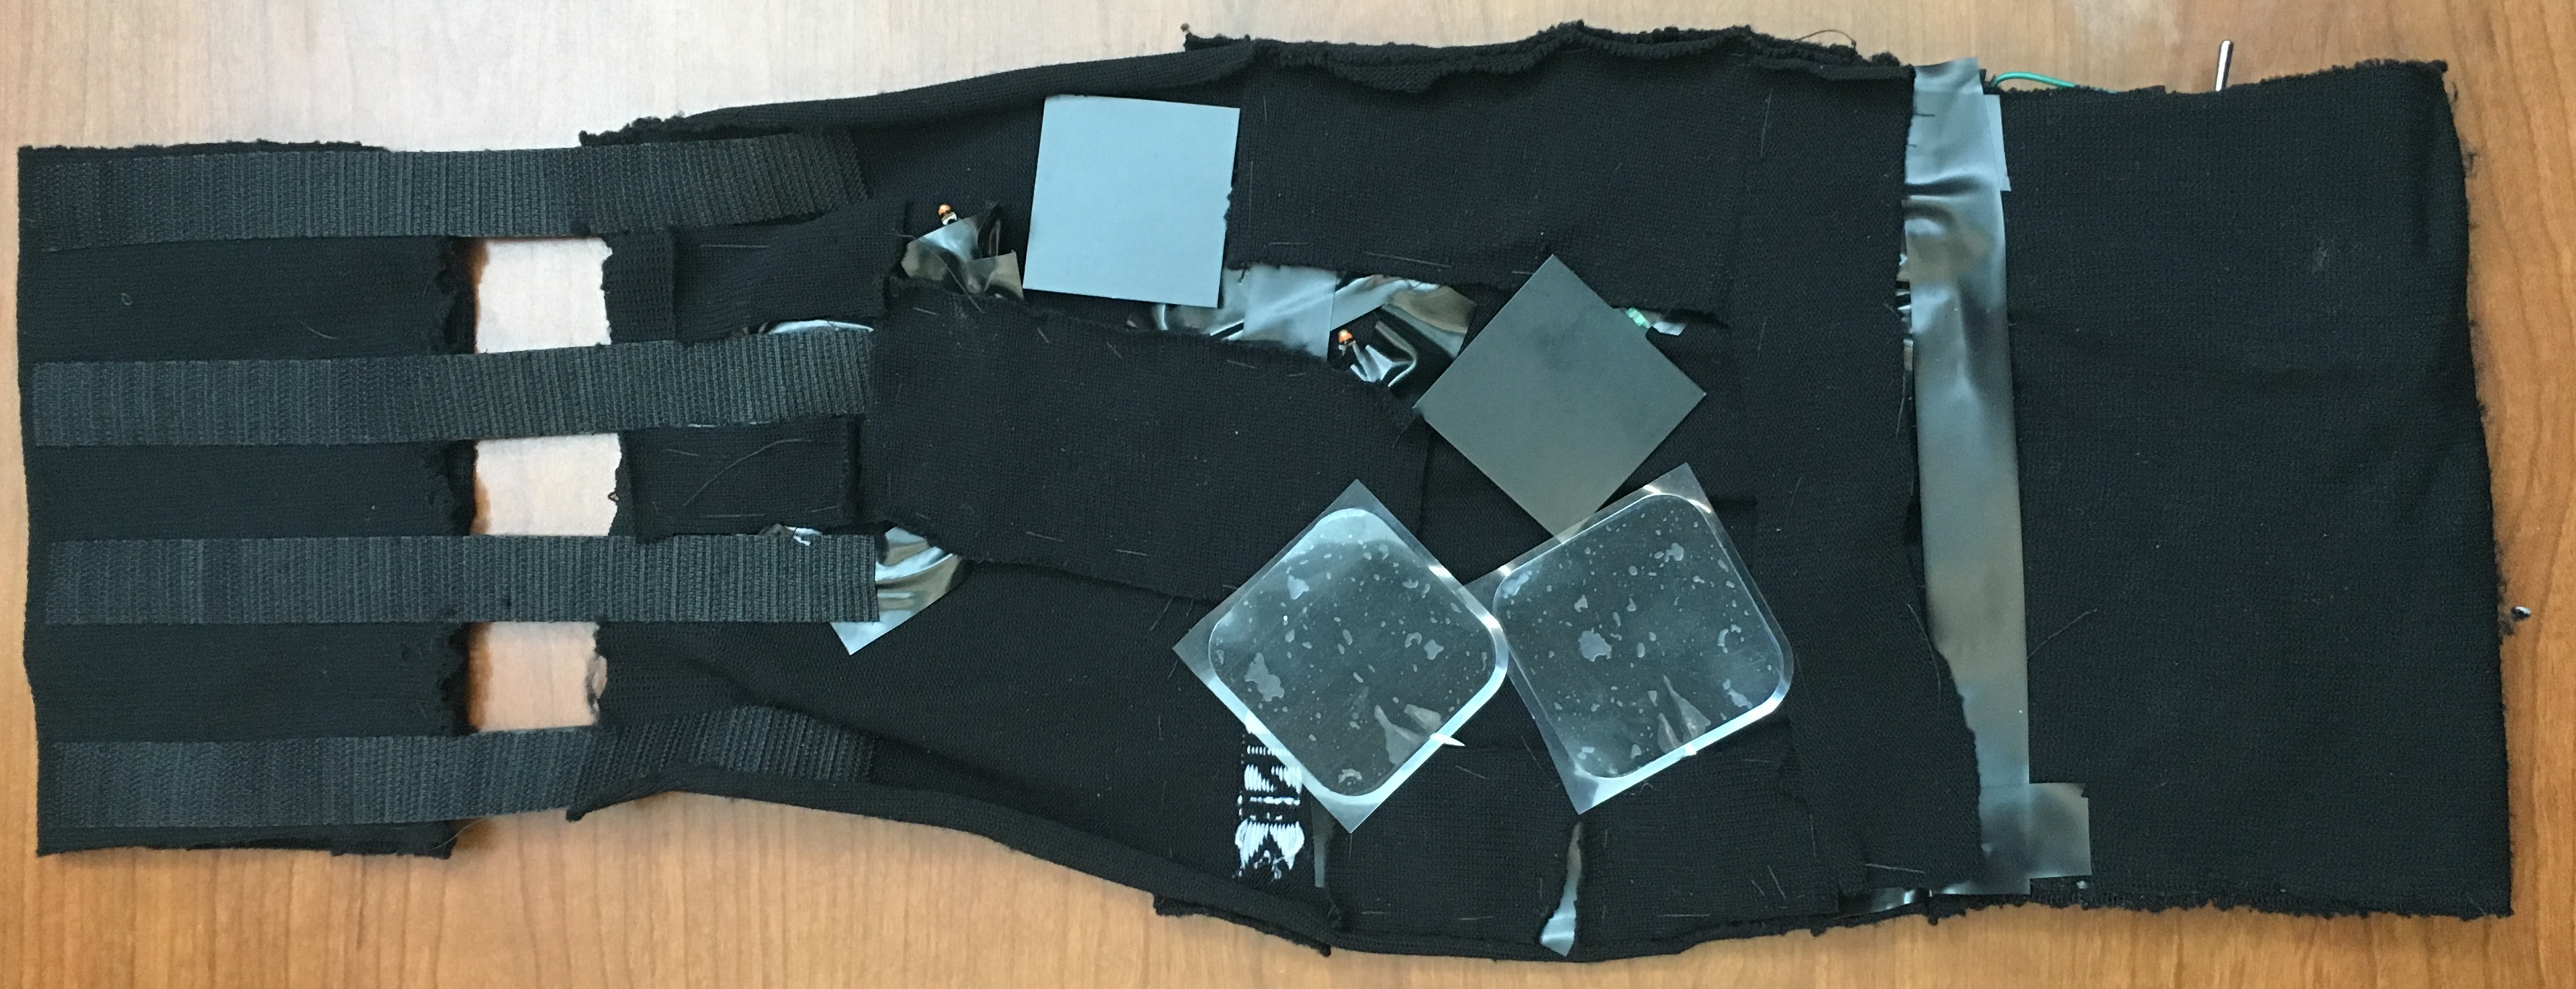
\includegraphics[width=0.9\linewidth]{titlepage/VDBand.JPG}
    \caption{VDBand Prototype}
    \label{fig:VDB}
\end{figure}
\vspace{0.5}

\subsection{Constraints and Criteria}
\textbf{Constraints}
\begin{itemize}
\item  \textbf{Safety}\\
The product was required to be safe and have have features that would mitigate any hazard imposed on user. The function was realized through the use of Nylon as the material of the product. Nylon is both sweat and water resistant, and acts as an electrical insulator. In the event that the circuit short circuited, the Nylon would be able to protect the user. 

\item \textbf{Architecture of the AdaFruit Flora}\\
The frequency of stimulation is limited by the operating frequency of the  micro controller that would be used. The frequency that the team chose to output the signal was around 5 Hz, while the frequency to induce muscle contraction is around 20-30 Hz at a 6V peak to peak level. The Flora operates at a clock cycle of 8 MHz which is more than needed to generate the square wave. Other constraints based on the parameters of the Flora include the size our program is allowed to be, and the voltage levels it is using. The Flash Memory size of the Flora is 16 KB, with 2 KB being used for the bootloader. Consequentially, programs can only be a maximum of 14 KB in size. The Flora is also using 3.3 V logic, and as such the voltage may have been inadequate to activate other components. 
\end{itemize}

\textbf{Criteria}
\begin{itemize}
\item \textbf{Weight of the Product}\\
The team designed the product with the intention of keeping it lightweight to prevent discomfort in the user. The components for the product, including the circuitry and micro controller contribute very little weight. The battery that was initially used contributed substantially to the weight. The total weight of the device including the battery was about 0.6 lbs. The weight aids in relieving any discomfort the user may feel when wearing the device. 

\item \textbf{Ease of Comfort}\\
The team focused on the VDBand being breathable and comfortable on the user. Nylon was used since it allowed the passing of air through itself. This would aid in the removal of heat from the afflicted area, since air is able to move over the skin. The sleeve is also highly flexible. The user is able to manually adjust the sleeve to match their comfort level. 

\end{itemize}

\subsection{Engineering Tools Used}
For the success of the project to be realized, a variety of software and hardware tools were utilized by the members of the group. The tools are listed as followed. 
\begin{itemize}
\item  \textbf{Arduino IDE (Arduino.cc, Ivrea, Italy, 2005)}\\
The Arduino IDE (Integrated Developemnt Environment) is an open source software that allows for the development of novel devices that can interact with the physical world. The IDE allows for the microcontroller development boards produced by the Arduino company to be programmed with relative ease even by those without any experience in programming. The IDE allows for rapid implementation and prototyping of a device. The Arduino code used to operate the VDBand can be referenced in Appendix A6. 

\item \textbf{Fritzing (Fritzing, Interaction Design Labs, Postdam, Germany, 2016)}\\
Fritzing is an open source CAD software package that allows for the digital construction of circuits using discrete components such as capacitors, resistors, and transistors or through the use of integrated chips such as the LM7805 Voltage Regulator or the 555 Timer chip. The components can be displayed either in schematic form, or layered on an actual breadboard or they can be placed onto a virtual PCB. The Fritzing software was used to create the circuit schematics and digrams for the device. 

\item \textbf{MATLAB (MathWorks, Massachussets, USA, 2018)}\\
MATLAB is a mathematical software package that allows for the extensive implementation of numerical methods, signal processing, and the simulation of dynamic models. The software features a variety of packages and libraries for tasks such as audio or image processing, or for tasks like regression analysis. The team used the package to create calibration curves for the sensors that were in the device.

\item \textbf{Soldiering Iron (Vaster, Denver, Colorado, USA, 2018)}\\
A soldering iron is used to join other components together by melting solder. A permanent bond is formed and the components are electrically conductive. The soldering iron allowed the team to create permanent attachments of the components to a perfboard. 

\item \textbf{Desoldering Pump (Vaster, Denver, Colorado, USA, 2018)}\\
The desolderig pump is used to remove excess solder or unusale solder from a PCB. The pump was used by the team to discard any unneccessary solder, or even solder that was just joined poorly.

\item \textbf{Heat Shrink Tubing (Gardener Bender, Menomonae Falls, Wisconsin, USA, 1959)}\\
Heat shrink tubing was used by the team to electrically insulate the exposed wires that were soldered together. A heat gun had to be applied to cause the tubing to thermally contract. 

\item \textbf{Wire Strippers (CAnadian Tire, Toronto, Ontario, Canada, 1922)}\\
Theses were used by the team to cut wires of a specific gauge size, and to strip them of their insulation so that they may be soldered. The device was used extensively when the circuit was being transferred from the breadboard to the perfboard.

\item \textbf{Solder Third Helping Hand (Elenco, Wheeling, Illinois, USA, 1972)}\\
The device keeps wires or PCBs in place as they are being soldered. The device has two mobile hands which can have their ease of movement adjusted via wing nuts, and the device also features a magnifying glasss. This was used extensively by the group during the soldering process. 


\end{itemize}




\section{Conclusion}
\subsection{Summary}
In conclusion the VDBand is a viable option for patients suffering from venous insufficiency problem. It was designed as a symptom relief instrument that is unlike any other treatment options on the market. The decision roots from the fact that varicose veins diagnosis is very easy based on qualitiatve assessment, so a device is not needed. Hence, neuromuscular electrical stimulation (NMES) was used to relieve the patient of symptoms, as it is a proven technique, and is also helping to address the root of the vein problem. \\

The design solution involves a compressive sleeve on the calf with detectors that look for the characteristics of varicose veins. The sensors used are thermistors (SEN00250) and force sensitive resistors (FSR406). Differential calculations were used to determine the characteristics, between an afflicted area of the calf, and a non-afflicted area. The two conditions to be satisfied are a temperature difference of 0.5\degree C, and 90mmHg, of systolic blood pressure. Once both of these conditions are satisfied, the device will proceed to apply neuromuscular electrical stimulation. This method would help aid in venous return by having muscle contractions. \\

An Adafruit Flora was used as the microcontroller as it is very small and compact, and generally used for wearable technology. The NMES pads have a gel interface to reduce the impedance between the skin and the contact pads. The NMES pads required a biphasic pulse in order to prevent the accumulation of charge on the skin, which can be detrimental to the health of the patient. Hence, and H-Bridge was used, with 4 MOSFETs. These transistors are good for a pulsing signal, and can achieve that at relatively high frequencies. The sensor data was collected onto the Flora, and constantly calculating the difference of the two parameters between the two points. This was considered the input circuit. The output circuit is the H-Bridge and the NMES pads. Once the two conditions were satisfied, an output signal was sent to apply a biphasic pulse from the H-Bridge, and send that to the NMES pads. \\

Because there are no therapeutic products like the VDBand currently on the market, it is a very marketable product. The only competition with this product are compression sleeves. As outlined above, the VDBand has far more capabilities and is more applicable than these compression sleeves. For this reason of novelty and uniqueness it can be marketed for a profit margin of about 300\%. Since it costs \$57.86 to manufacture, it can be sold for \$175. In terms of product manufacturing, an analysis was performed to show that it is economically wiser to start a new manufacturing facility, rather than outsourcing it and have it produced by another party. If the product was commercialized, some losses are expected, as there are many start-up costs involved. However, this product is expected to be a well desired product due to its applications, and usability. Hence, profits are projected to increase drastically and prove to be economically feasible. \\

The VDBand will be marketed mainly with social media and television advertisements to appeal to the target market, of adults, pregnant women, and people that are overweight. Television advertisements are shown to appeal to the adult population greatly, and social media is widely used now, so it's very easy to target these groups of people. The product is also a reliable option because it has a very long life cycle. It is very robust, but can't be used beyond it's limits, such as use in water, as it can fry the circuits. If anything does happen to the VDBand, it can be easily sent back to the manufacturer for repair.\\

\subsection{Future Recommendations}
The product created in this initial stage is simply a prototype and can be expanded to much more, based on the same principles. It definitely has great potential for success, and beneficial applications to many people. 

\begin{itemize}
    \item The VDBand can be made waterproof or washable, as sanitation may be a concern of some users. For example, the use of nylon has the benefit of being able to wick up sweat, so there will be sweat present in the sleeve. Since there are electrical components and wires in the product, it would be difficult to make it washable, without creating a safety hazard. Hence, it can be housed in a plastic material on the outside to protect all the electrical components and keep it waterproof. Another way to work around this is to make the main electrical circuits removable, so that the fabric can be washed. This solution may require further development, as there are wires to interface the sensors with the microcontroller, so these would be left hanging when removing the circuits. The use of jumper cables would make this solution more feasible and remove the clutter of wires. 
    
    \item A control system can be implemented, which allows the user to control the amplitude and frequency of the electrical pulses that are applied. This is more effective than just a set value, because severity and comfort varies immensely amongst persons. NMES systems right now have a large bulky unit with an LCD display that allow users the set the parameters of the NMES. In order to keep the VDBand compact, a wireless module can be added to the system, and the parameters would be controlled by a user-friendly phone app. This would increase user-friendliness and make it applicable to a wider sample of patients. 
    
    \item Since all these sensors and components are subject to wear and tear, the sensors should be removable and easily replaceable. This can also be achieved using wire headers so that it is easily accessible for the patients, and reduces the stresses of having to contact the company and send it in for repair. This is a simple recommendation, but can be of satisfactory quality if commercialized. Another safety factor to be considered is the heating of the battery due to high frequency pulses produced by the NMES pads. A regular 9V Lithium Ion battery is not meant for high frequency applications, so a Lithium Polymer battery would be better to use in order to prevent overheating. This can cause discomfort on the patient when the battery heats up, it can fry the circuitry, and can also inadvertently satisfy the temperature threshold, creating the possibility for an unnecessary triggering of the NMES system. This can also further promote unnecessary inflammation in the bulging veins, creating adverse health effects on the patient's leg. 
    \item Deep learning networks can be implemented in the product to make the system adapt to different modes of activity that the user may be in. Pressure and temperature thresholds may change if a person is sleeping, or resting, or running. The idea with this recommendation is to train the system to recognize these activities, and then load a particular set of thresholds that will trigger the NMES. In order to do this, other sensors may also be required such as gyroscopes and heart rate monitors. The system then needs to be trained to recognize these situations based on comparisons to a library of parameters. 
\end{itemize}

\subsection{Future Research}
Before actually using the product, extensive tests still need to be performed on test subjects. There needs to be further validation that the blood pressure and temperature thresholds are reliable values to trigger the NMES. This would be done by performing studies on multiple varicose veins patients and observing the pressure and temperature differentials between an afflicted and non-afflicted area in the lower extremities. Statistical measures can then be performed in order to determine a better researched set of  threshold values. In current tests, varicose veins conditions were simulated, but wasn't actually tested on a varicose veins subject. So, testing on actual patients will not only give us more accurate threshold values, but also test the effectiveness of the detection system of the instrument. \\

Another test that needs to be performed is the effectiveness of the NMES therapy along with the natural  compression of the sleeve itself. This needs to be done by applying the muscle stimulation at the correct levels and then assessing the condition of the calf veins after the stimulation. It is proven in literature to be an effective relief of symptoms, but having the experimental validation would really help the reliability of the VDBand. 


\pagebreak
\begin{thebibliography}{9}

\bibitem{CVC}
Canadaveinclinics. (2018). \textit{Vein conditions}. [Online]. Available at: http://www.canadaveinclinics.ca/vein-conditions/. [Accessed November 24, 2018].

\bibitem{CSVS}
J. Dooner, \textit{VARICOSE VEINS}. [Online]. Available at: https://canadianvascular.ca/Varicose-Veins. [Accessed November 24, 2018].

\bibitem{CSVS2}
Canadaveinclinic. (2018). \textit{Varicose Veins}. [Online]. Available at: http://www.canadaveinclinics.ca/vein-conditions/varicose-veins/. [Accessed November 24, 2018].

\bibitem{Treatment}
Gloviczki, P., Comerota, A., Dalsing, M., Eklof, B., Gillespie, D., Gloviczki, M., Lohr, J., McLafferty, R., Meissner, M., Murad, M., Padberg, F., Pappas, P., Passman, M., Raffetto, J., Vasquez, M. \& Wakefield, T. (2011). The care of patients with varicose veins and associated chronic venous diseases: Clinical practice guidelines of the Society for Vascular Surgery and the American Venous Forum. \emph{Journal of Vascular Surgery}. 53(5), pp. 25-48.

\bibitem{Shaydakov}
Shaydakov, M.E. \& Diaz, J.A. (2017). Effectiveness of infrared thermography in the diagnosis of deep vein thrombosis: an evidence-based review. \emph{Journal of Vascular Diagnostics and Interventions}. 5(1), pp. 7-14.

\bibitem{Rohan}
Rohan, C.P-Y., Badel, P., Lun, B., Rastel, D., \& Avril, S. (2013). Biomechanical response of varicose veins to elastic compression. \emph{Journal of Biomechanics}. 2013(46), pp. 599-603.

\bibitem{press2}
Bradbury, A.W. (2011). Mechanisms of Vascular Disease. South Australia: University of Adelaide Press.

\bibitem{Doucet}
Doucet, B.M., Lam, A. \& Griffin, L. (2012). Neuromuscular Electrical Stimulation for Skeletal Muscle Function. \emph{Yale J Biol Med}. 85(2), pp. 201-215.

\bibitem{JCN}
Franz, A. \& Wann-Hansson, C. (2015). Patients’ experiences of living with varicose veins and management of the disease in daily life. \emph{Journal of Clinical Nursing}. 25(5-6), pp. 733-741.

\bibitem{UK}
National Clinical Guideline Centre (UK). \textit{NICE Clinical Guidelines}. [online]. Available at: https://www.ncbi.nlm.nih.gov/books/NBK328029/. July 2013. 

% LIT REVIEW
\bibitem{Sell}
Sell, H., Vikatmaa, P., Alback, A., Lepantalo, M., Malmivaara, A., Mahmoud, O. \& Venermo, M. (2014). Compression Therapy Versus Surgery in the Treatment of Patients with Varicose Veins: A RCT. \emph{European Journal of Vascular and Endovascular Surgery}. 47(6), pp. 670-677.

\bibitem{Willenburg}
Willenberg, T. (2014). Treatment of varicose veins. \emph{Reviews in Vascular Medicine}. 2014(2), pp. 67-72.

\bibitem{Gunn}
Noble, J., \& Gunn, A.A. (1972). VARICOSE VEINS: COMPARATIVE STUDY OF METHODS FOR DETECTING INCOMPETENT PERFORATORS. \emph{The Lancet}. 1972(June), pp. 1253-1255.

\bibitem{Usamentiaga}
Usamentiaga, R. \& Garcia, D.F. (2017). Infrared Thermography Sensor for Temperature and Speed Measurement of Moving Material. \emph{Sensors}. 17(1), pp. 1157-1178.

\bibitem{Herbert}
Herbert, J. (2003). The principles of neuromuscular electrical stimulation. \emph{Advanced Practice Continence Supplement}. 99(19), pp. 54-55.

\bibitem{Ravikumar}
Ravikumar, R., Babber, A., Lane, T.R., Moore, H.M. \& Davies, A.H. (2017). Randomised Controlled Trial: Potential Benefit of a Footplate Neuromuscular Electrical Stimulation Device in Patients with Chronic Venous Disease. \emph{Eur J Vasc Endovasc Surg}. 53(1), pp. 114-121.

\bibitem{Son}
Son, J., Lee, D., \& Kim, Y. (2014). Effects of involuntary eccentric contraction training by neuromuscular electrical stimulation on the enhancement of muscle strength. \emph{Clincal Biomechanics}. 2014(29), pp. 767-772.

\bibitem{Maughan}
Maughan, R.J., Watson, J.S. \& Weir, J. (1983). Strength and cross-sectional area of human skeletal muscle. \emph{J. Physiol}. 338(1), pp. 37-49). 

\bibitem{Narayana}
Narayana, H., Hu, J., Kumar, B., Shang, S., Ying, M. \& Young, R.J. (2018). Designing of advanced smart medical stocking using stress-memory polymeric filaments for pressure control and massaging. \emph{Materials Science \& Engineering}. 91(1), pp. 263-273.

% References in MOTIVATION section

\bibitem{Mayo}
Mayoclinic.org. (2018). \textit{Varicose veins - Diagnosis and treatment - Mayo Clinic.} [online] Available at: https://www.mayoclinic.org/diseases-conditions/varicose-veins/diagnosis-treatment/drc-20350649 [Accessed 30 Nov. 2018].

\bibitem{Zensah}
Zensah. (2018). \textit{Why Do Athletes, Runners Wear Leg Compression Sleeves?.} [online]. Available at: https://www.zensah.com/pages/why-wear-leg-compression-sleeves [Accessed 30 Nov. 2018].

\bibitem{Antisatax}
Antistax.ca. (2018). \textit{Tablets with red vine leaf extract - Antistax® Canada.} [online]. Available at: https://www.antistax.ca/en/product/how-antistax-works/red-vine-leaf-extract.html [Accessed 30 Nov. 2018].

\bibitem{Axio}
AxioBionics. (2018). \textit{The Upper Extremity Biosleeve.} [online]. Available at: http://axiobionics.com/ue-biosleeve/ 

\bibitem{MedNews}
University of Illinois-Chicago, S. (2018). \textit{Varicose veins: Causes, treatment, diagnosis, and prevention.} [online]. Medical News Today. Available at: https://www.medicalnewstoday.com/articles/240129.php [Accessed 30 Nov. 2018].

\bibitem{Healthy}
Healthywomen.org. (2018). \textit{Varicose Veins | HealthyWomen.} [online]. Available at: https://www.healthywomen.org/condition/varicose-veins [Accessed 30 Nov. 2018].

\bibitem{ACBJ}
Bizjournals.com. (2018). [online]. Available at: https://www.bizjournals.com/tampabay/news/2018/11/ 15/jabil-partners-with-med-tech-startup-on-devices.amp.html?fbclid=IwAR29a1fGpD74\_3wg66nSzZjti2 PhqRpX7Md2xPsGmkMftx856wmtfTs4\_Ls [Accessed 30 Nov. 2018].

\bibitem{Stats}
Average weekly time spent watching television in Canada from 2016/2017 to 2017/18 broadcast year, a. (2018). textit{Canada weekly time spent with TV by age 2018 l Statistic.} [online]. Statista. Available at: https://www.statista.com/statistics/234311/weekly-time-spent-watching-tv-in-canada-by-age-group/ [Accessed 30 Nov. 2018].

\bibitem{FSB}
Aland, M. (2018). \textit{Local \& National TV Advertising Costs \& How to Advertise 2017.} [online]. Fit Small Business. Available at: https://fitsmallbusiness.com/tv-advertising/ [Accessed 30 Nov. 2018].

\bibitem{ATL}
Madrigal, A. (2018). \textit{When Did TV Watching Peak?.} [online]. The Atlantic. Available at: https://www.theatlantic.com/technology/archive/2018/05/when-did-tv-watching-peak/561464/ [Accessed 30 Nov. 2018]. 

\bibitem{AYCR}
All You Can Read. (2018). \textit{Top 10 celebrity magazines.} [online]. Available at: https://www.allyoucanread.com/top-10-celebrity-magazines/ [Accessed 30 Nov. 2018].

\bibitem{ELE}
Event Log Explorer. (2018). \textit{Event Log Explorer.} [online]. Available at: https://eventlogxp.com/blog/saving-event-logs-to-one-event-log-file/ [Accessed 23 Nov. 2018].

%\bibitem{Clker}
%Clker.com. (2018). \textit{Factory Clip Art at Clker.com - vector clip art online, royalty free & public domain.} [online]. Available at: http://www.clker.com/clipart-1773.html [Accessed 30 Nov. 2018].

%\bibitem{Vector}
%Vector.me. (2018). \textit{Logs.} [online]. Available at: https://vector.me/browse/146342/brown$_$box$_$paper$_$cartoon$_$package$_$cardboard$_$closed$_$boxes$_$taped [Accessed 23 Nov. 2018].

\bibitem{SSSL}
Londonstorage.wordpress.com. (2018). \textit{Storage Services | Self Storage Services London | Page 2.} [online]. Available at: https://londonstorage.wordpress.com/category/home/storage-services/page/2/ [Accessed 30 Nov. 2018].

\bibitem{All}
ARTICLES, T., PRODUCTS, N., ELECTRONICS, G., PROJECTS, C., MICRO, E., Lectures, V., Webinars, I., Training, I., Search, P., DB, T., Tool, B. and Designs, R. (2018). Pulse Width Modulation | DC Motor Drives | Electronics Textbook. [online] Allaboutcircuits.com. 
Available at: https://www.allaboutcircuits.com/textbook/semiconductors/chpt-11/pulse-width-modulation/ [Accessed 18 Nov. 2018].

\bibitem{Ada}
Industries, A. (2018). FLORA - Wearable electronic platform: Arduino-compatible. [online] Adafruit.com. Available at: https://www.adafruit.com/product/659 [Accessed 18 Nov. 2018].

%\bibitem{Freepik}
%Freepik. (2018). \textit{recycle symbol.} [online]. Available at: https://www.freepik.com/free-icon/recycle-symbol$_$755408.htm [Accessed 30 Nov. 2018].

%\bibitem{VectorS}
%Vectors, R., Vectors, C. and Image, T. (2018). \textit{Trash can icon cartoon style vector image on VectorStock.} [online]. VectorStock. Available at: https://www.vectorstock.com/royalty-free-vector/trash-can-icon-cartoon-style-vector-12136853 [Accessed 30 Nov. 2018].

%\bibitem{FreeVectors}
%All-free-download.com. (2018). \textit{Downloadcartoon tools 04 vector 180575 free vector download (224,116 Free vector) for commercial use. format: ai, eps, cdr, svg vector illustration graphic art design.} [online]. Available at: https://all-free-download.com/free-vector/download/cartoon-tools-04-vector$_$180575.html [Accessed 30 Nov. 2018].

%\bibitem{clipart}
%Person Outline Printable. (2018). \textit{Clipart | Free download best Ot Clipart on ClipArtMag.com.} [Online]. Available: http://clipartmag.com/person-outline-printable#person-outline-printable-1.jp. [Accessed: 30-Nov-2018].

%\bibliographystyle{clipartpen}
%Cartoon Truck Png Clipart Car Images In Png Moving Truck Clipart #58170 « ClipartPen. (2018). \textit{ClipartPen.} [Online]. Available: http://clipartpen.com/clipart-pen/cartoon-truck-png-clipart-car-images-in-png-58170.[Accessed: 30-Nov-2018].

% referneces in marketing section

\end{thebibliography}

\newpage

\pagenumbering{arabic}% resets `page` counter to 1
\renewcommand*{\thepage}{A\arabic{page}}
\appendix 
\newpage

\section{Appendix}
\subsection{Circuit Diagram}
\begin{figure}[!ht]
    \centering
    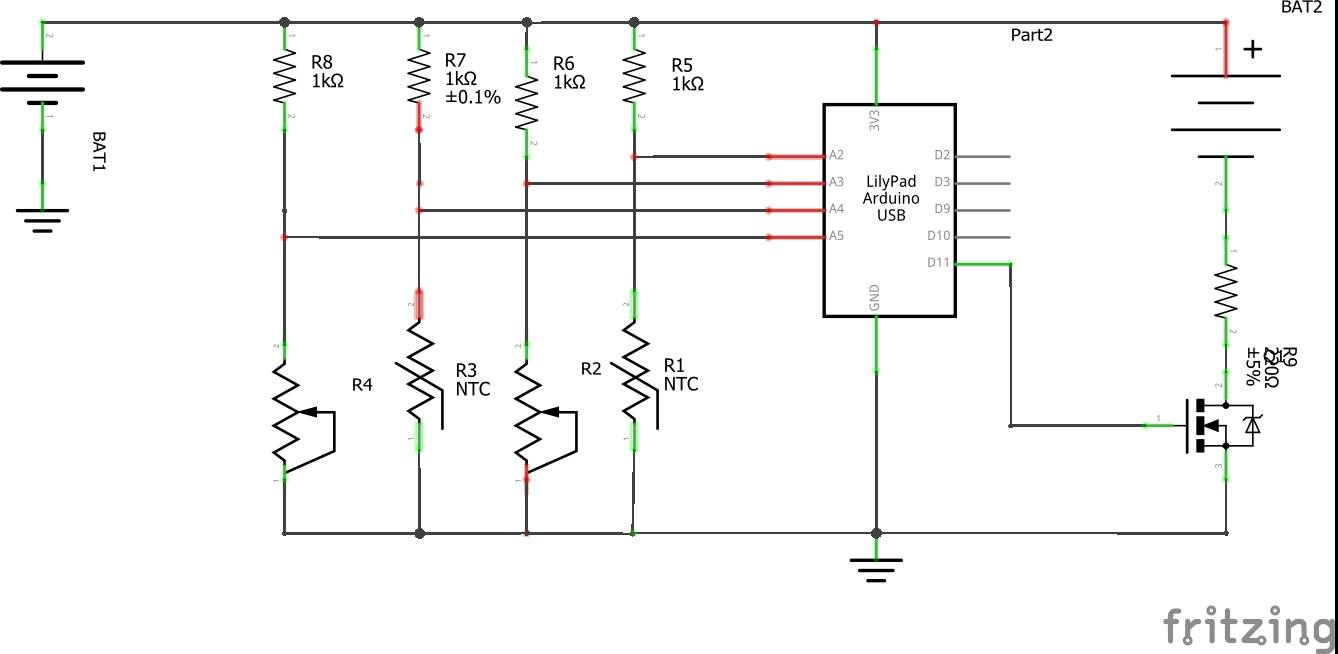
\includegraphics[width=0.9\linewidth]{Appendix/circuit.jpg}
    \caption{Original Circuit Diagram for the VDBand}
    \label{fig:circuit}
\end{figure}
\vspace{0.5mm}
\newpage

\subsection{Revised and Final Circuit}
\begin{figure}[!ht]
    \centering
    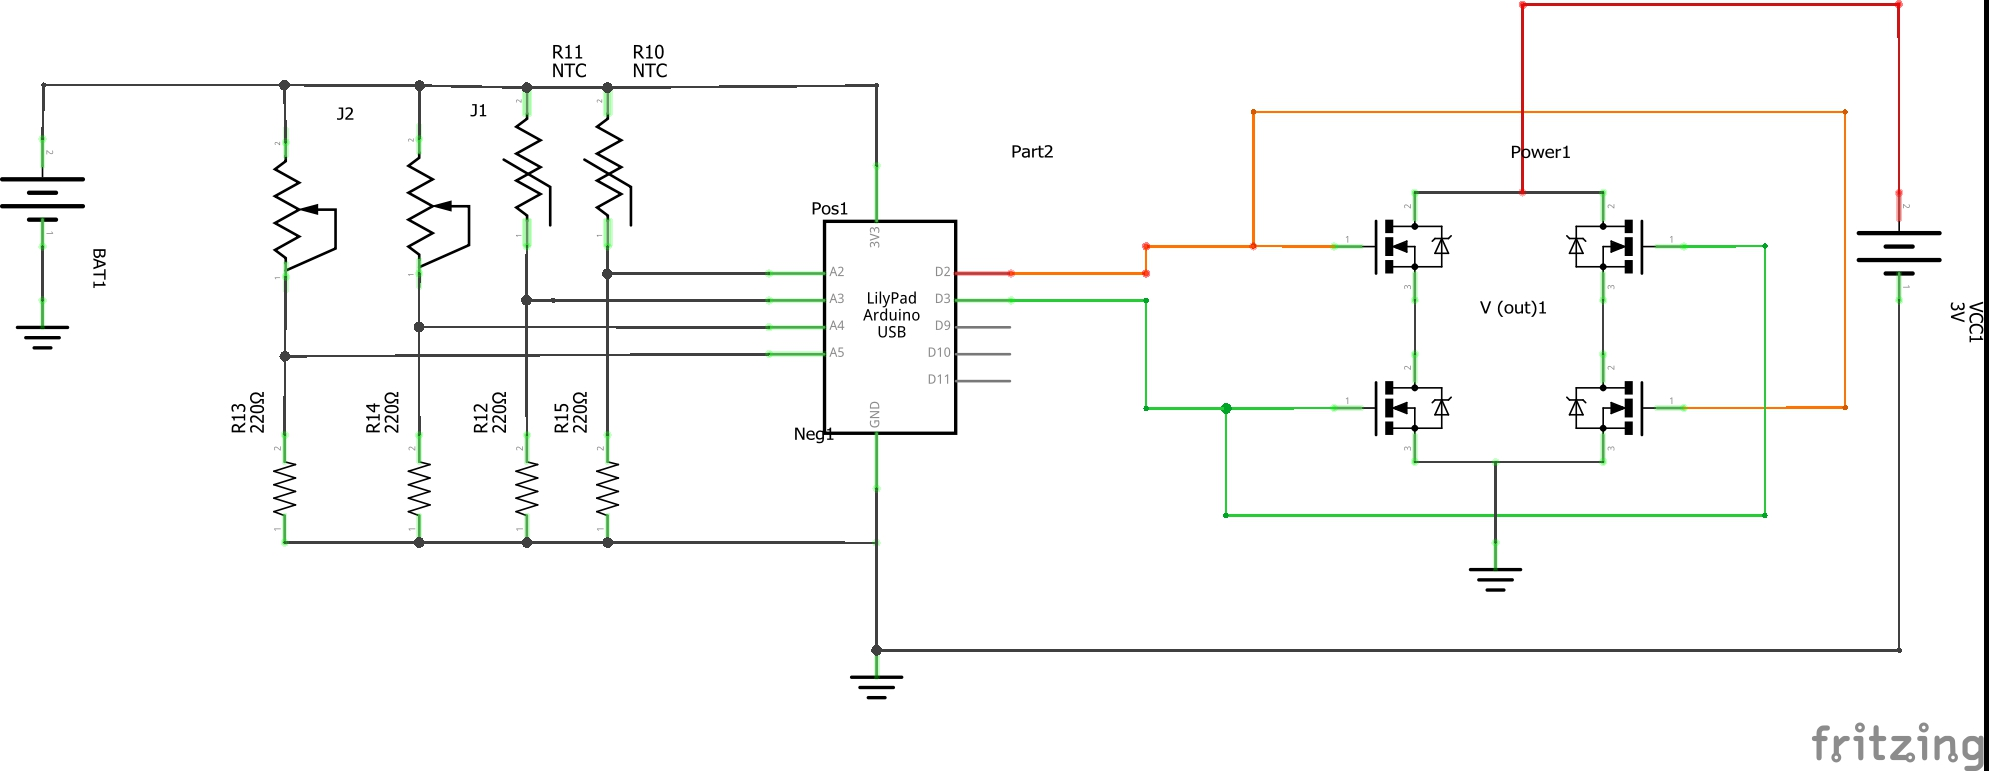
\includegraphics[width=0.9\linewidth]{Appendix/Updated.jpg}
    \caption{Final Circuit Diagram for the VDBand}
    \label{fig:IO}
\end{figure}
\vspace{0.5mm}
\newpage

\subsection{Input-Output Conversions}
\begin{figure}[!ht]
    \centering
    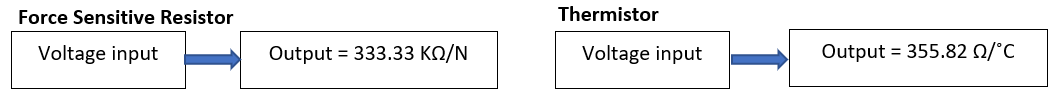
\includegraphics[width=0.9\linewidth]{Appendix/IO.PNG}
    \caption{Input-Output Conversions}
    \label{fig:IO}
\end{figure}
\vspace{0.5mm}
\newpage

\subsection{Circuitry}
\begin{figure}[!ht]
    \centering
    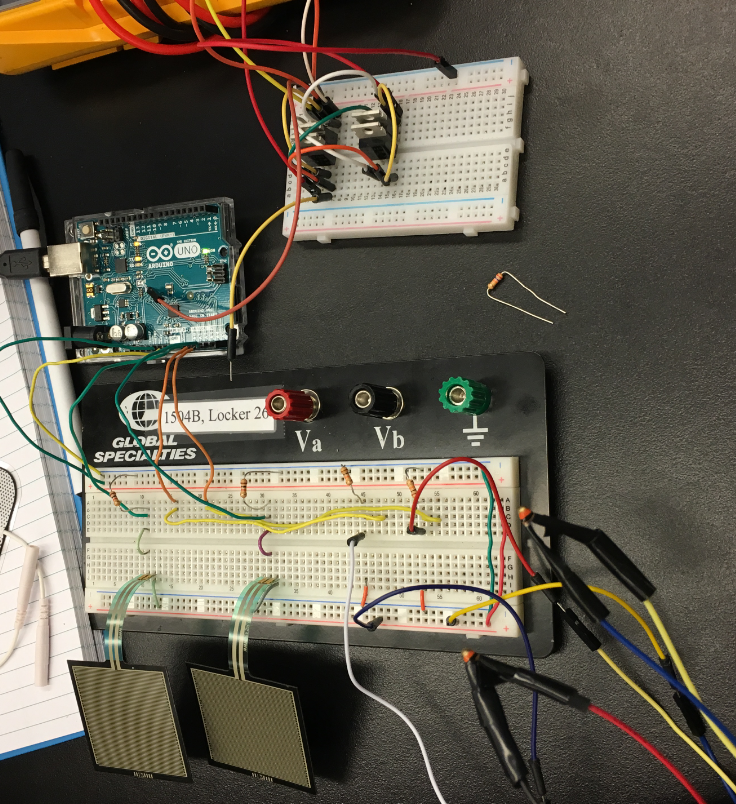
\includegraphics[width=0.9\linewidth]{Appendix/circuitry.PNG}
    \caption{Circuitry inside the VDBand}
    \label{fig:C}
\end{figure}
\vspace{0.5mm}
\newpage

\subsection{Components Used}
\begin{figure}[H]
    \centering
    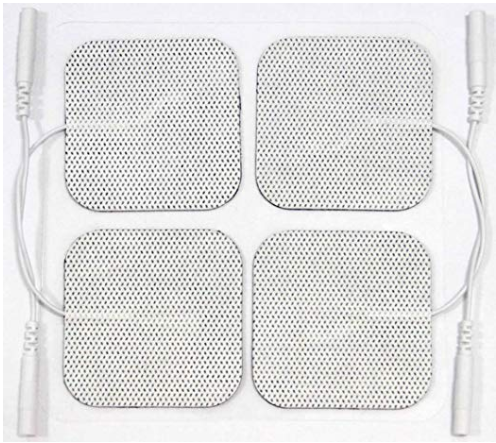
\includegraphics[width=0.5\linewidth]{Appendix/EMSP.PNG}
    \caption{Neuromuscular Electrical Stimulation Pads}
    \label{fig:EMSP}
\end{figure}
\vspace{0.5mm}

\begin{figure}[H]
    \centering
    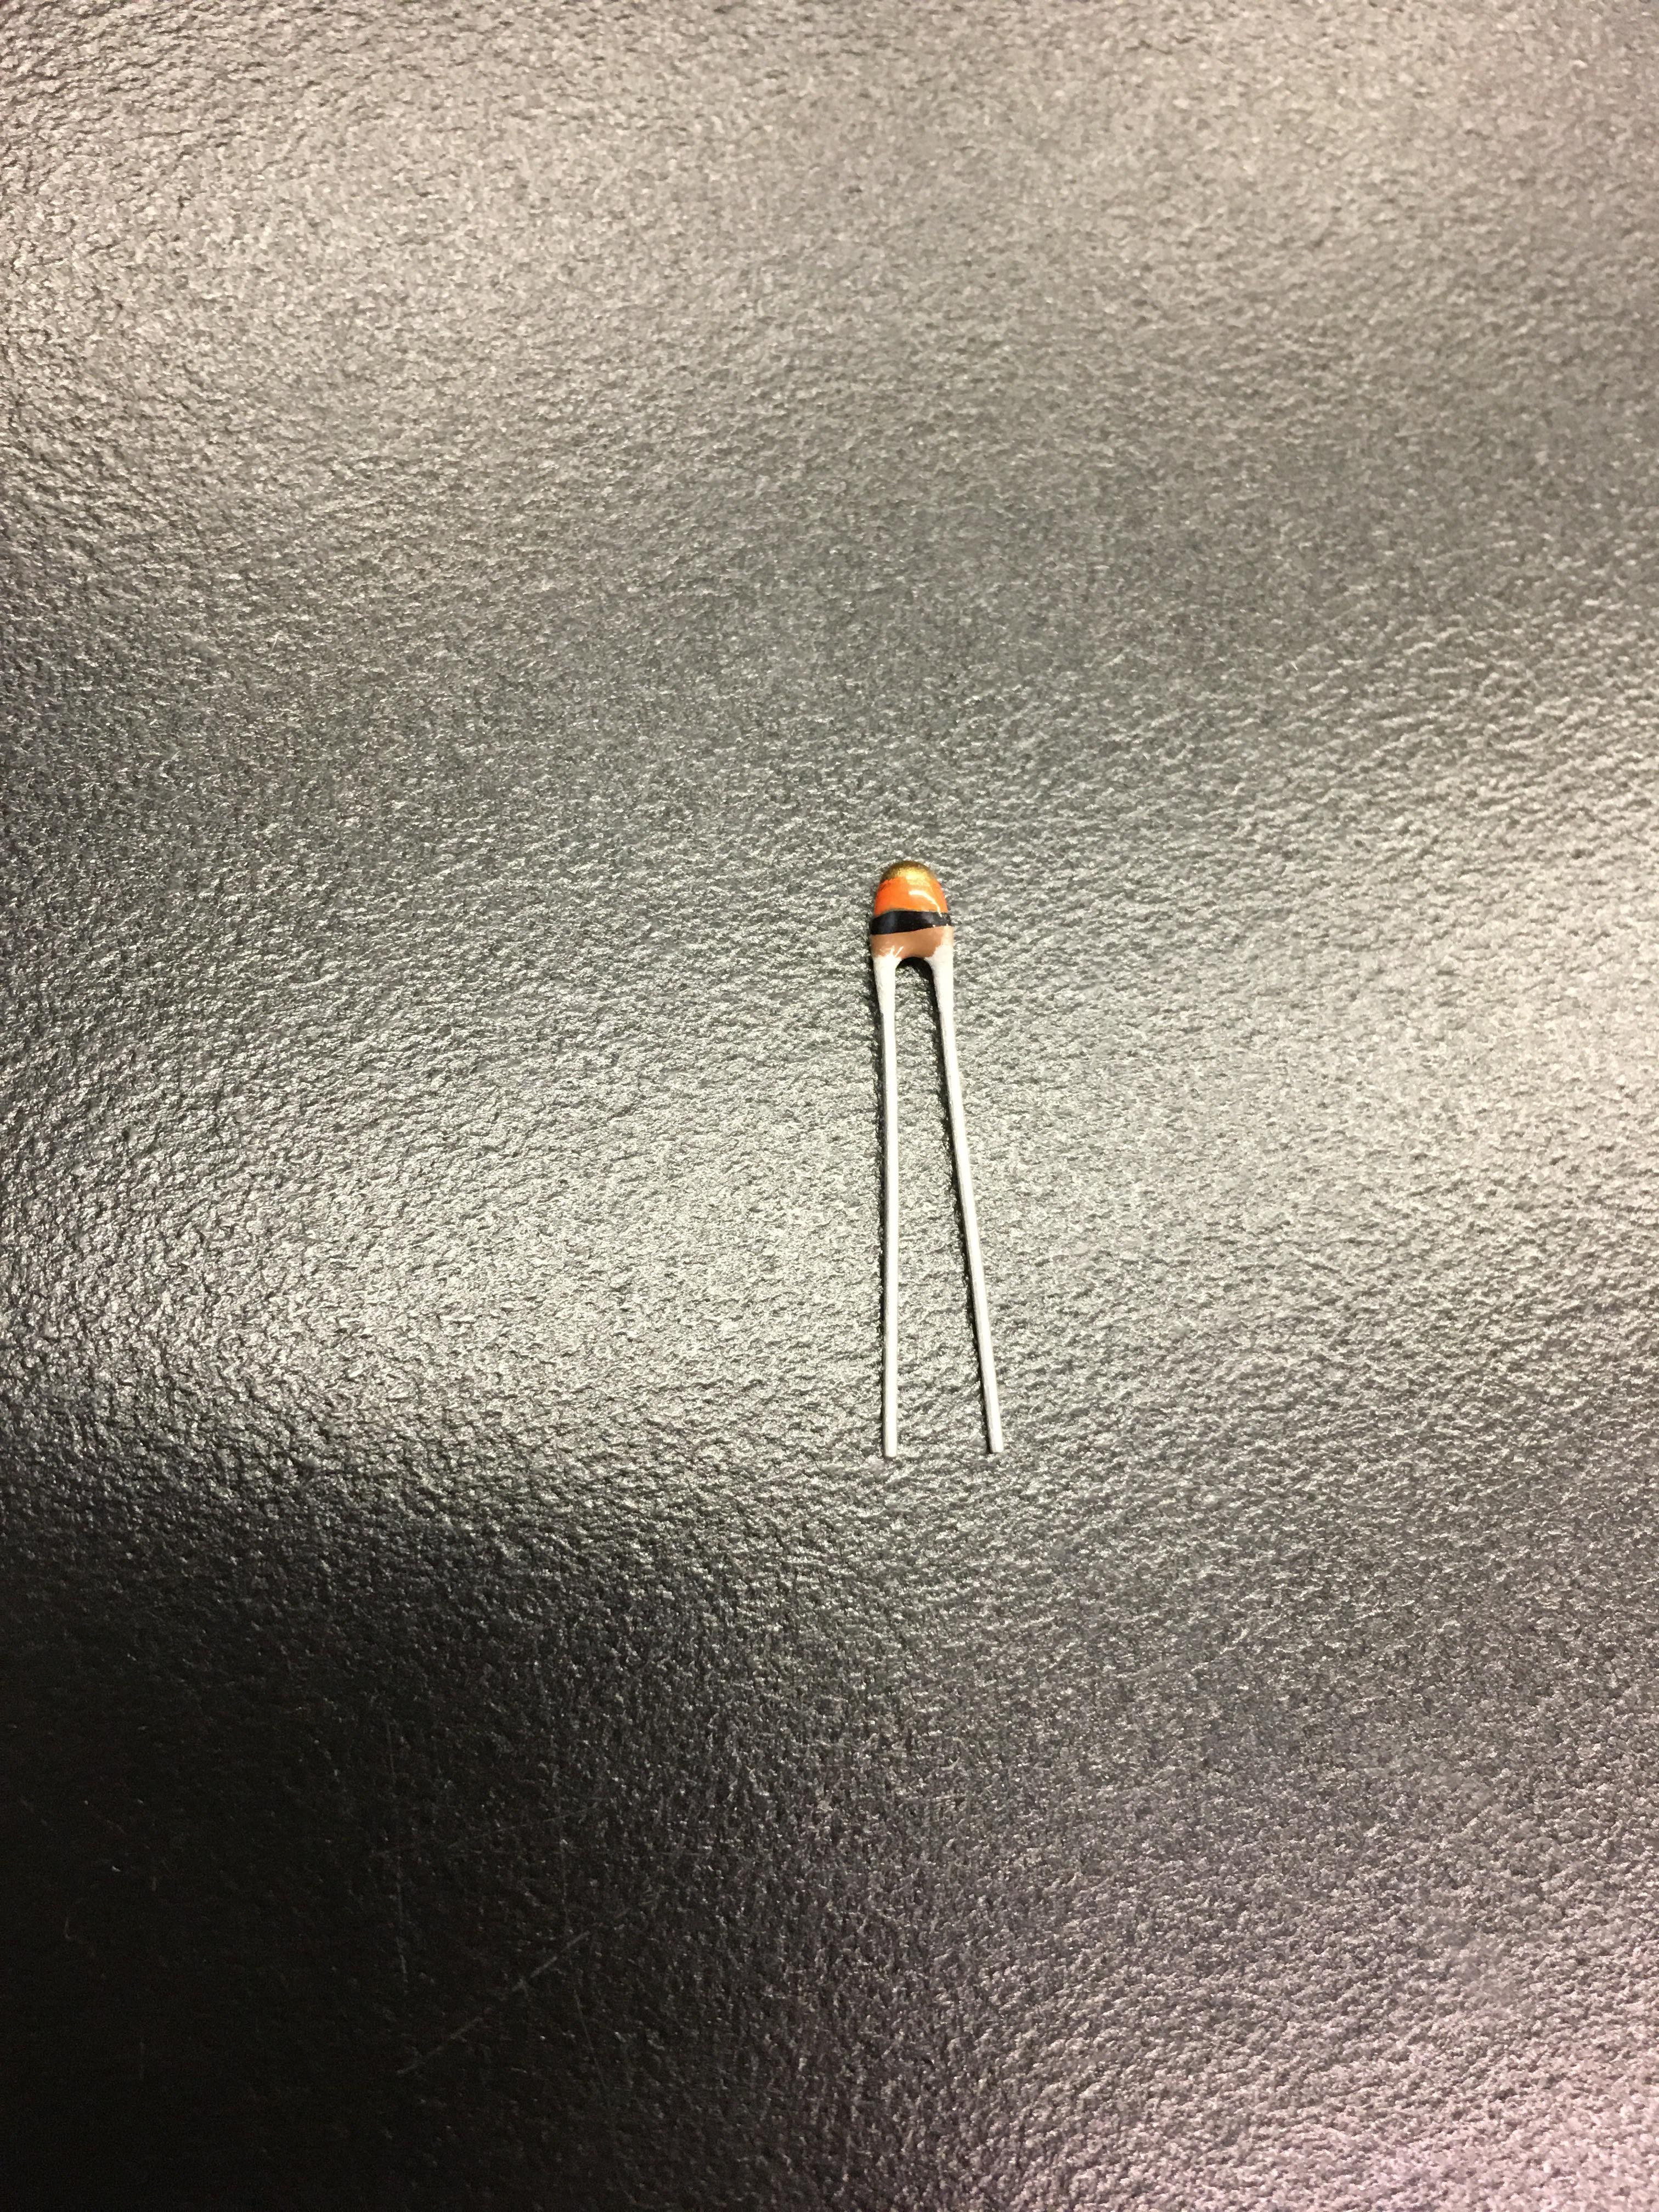
\includegraphics[width=0.5\linewidth]{Appendix/THERM.jpg}
    \caption{Thermistor}
    \label{fig:therm}
\end{figure}
\vspace{0.5mm}

\newpage

\begin{figure}[H]
    \centering
    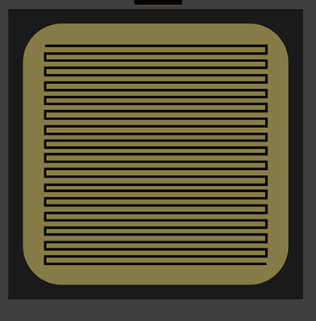
\includegraphics[width=0.5\linewidth]{Appendix/FSR.PNG}
    \caption{Force Sensitive Resistor}
    \label{fig:FSR}
\end{figure}
\vspace{0.5mm}

\begin{figure}[H]
    \centering
    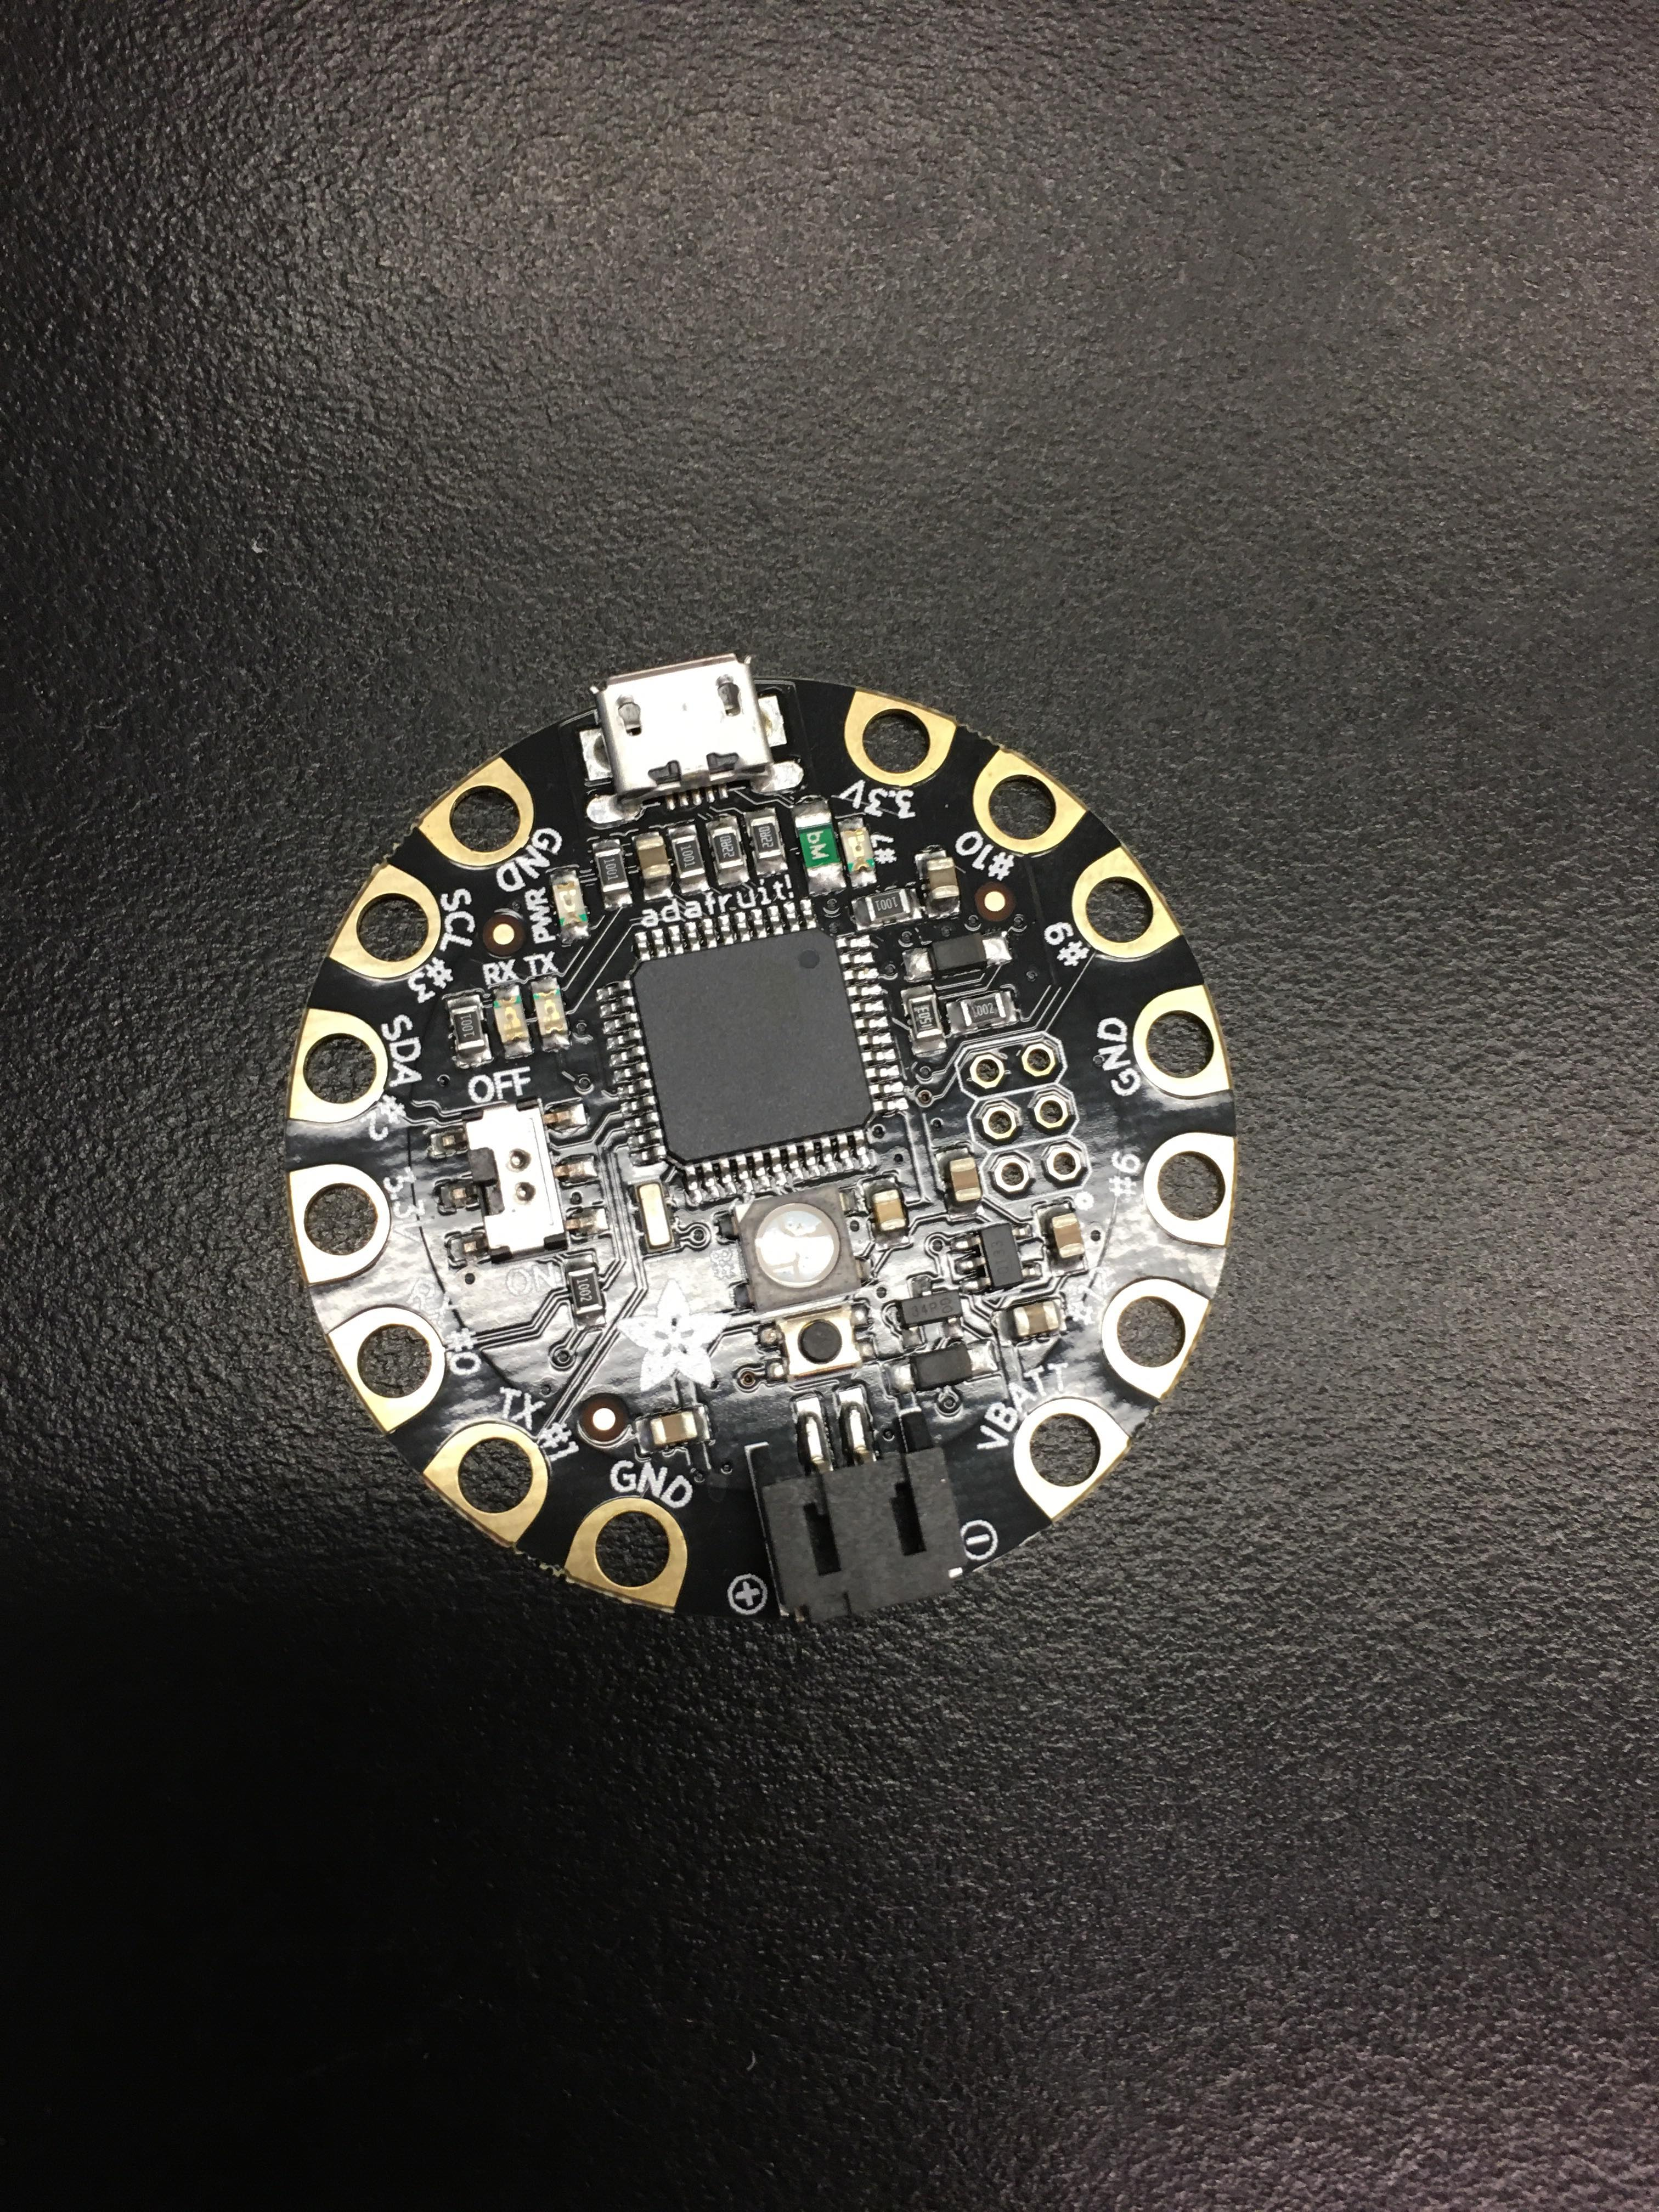
\includegraphics[width=0.5\linewidth]{Appendix/LP.jpg}
    \caption{Flora}
    \label{fig:LP}
\end{figure}
\vspace{0.5mm}\\

\newpage


\subsection{ Arduino Code} \label{D}
\subsubsection{D1 - Listing 1: FSR.ino}\label{D1}
\lstinputlisting[language=C, style= Matlab-editor, basicstyle = \scriptsize, caption= {FSR.ino}]{Scripts/FSR.ino}

\pagebreak

\subsubsection{Listing 2: FSR.ino} \label{D2}
\lstinputlisting[language=C, style= Matlab-editor, basicstyle = \scriptsize, caption= {FSR2.ino}]{Scripts/FSR2.ino}

\pagebreak

\subsubsection{Listing 3: OUTPUT.ino} \label{D3}
\lstinputlisting[language=C, style= Matlab-editor, basicstyle = \scriptsize, caption= {OUTPUT.ino}]{Scripts/Output.ino}

\pagebreak

\subsubsection{Listing 4: Thermistor.ino} \label{D4}
\lstinputlisting[language=C, style= Matlab-editor, basicstyle = \scriptsize, caption= {Thermistor.ino}]{Scripts/Thermistor.ino}

\pagebreak

\subsubsection{Listing 5: Thermistor2.ino} \label{D5}
\lstinputlisting[language=C, style= Matlab-editor, basicstyle = \scriptsize, caption= {Thermistor_2.ino}]{Scripts/thermistor_2.ino}

\end{document}